\documentclass{mathnote}
\usepackage{mathnote}


\begin{document}

% タイトルページの呼び出し
\tituloum{数学のノート}{Namachan}{}{}{\today}

%\include{Preambulo/Capa}

\cleardoublepage
\pagenumbering{arabic}
\pagecolor{white}

% 目次の表示
\localtableofcontents


\phantomsection
\part{用語の定義}

\begin{abstract}
  この章では，数学の学習を始める前に，定義・命題・定理・補題・系などの基本的な用語について理解を深める．「『命題』という言葉は知っているけど，『定理』とはどう違うの？」という疑問を持ったり，「『定義』と『定理』の違いがあやふやなままで，よくわからない」と感じる学生は多い．まず，日常的な例と数学的な例をもとに「定義」の性質を確認する．次に，命題・定理・補題・系という用語を整理し，これらのラベルの使い分けについて注意を述べる．最後に，「かつ・または」「とる・おく・固定する」「十分大きい」など，数学に特有の言い回しを具体例とともに確認しよう．
\end{abstract}

\phantomsection
\section{定義・命題・定理・補題・系}

\phantomsection
\subsection{定義}

数学用語には細かな意味がある．概要にも述べたように，「定義」と「定理」の違いなどをはっきりと認識しておくことは，
数学の学習を進める上で堅固たる「理解の基盤」となる．まずは「定義」の意味の確認からはじめよう：

\emph{定義}\index{ていぎ@定義}（\emph{definition}）とは，用語の意味を明確に述べたものであり，\textbf{Def}と略記される．
要するに「定義」とは，「この数学的概念（用語）はこのような意味である」という取り決めである．
数学のお話にうつる前に，日常的な「定義」の例を見てみよう．

\begin{example}{アレニウスによる酸・塩基の定義}{アレニウスによる酸・塩基の定義}
  水溶液中で水素イオン\ce{H+}を放出する物質を酸，\ce{OH-}を放出する物質を塩基とする．
\end{example}

\begin{example}{「民主主義」の定義}{「民主主義」の定義}
  民主主義とは，国民が政治の意思決定に直接または間接的に参加する政治体制のことをいう．
\end{example}

どちらもわかりやすい例であり，「すでに知っていること」と思われる読者もいるかもしれない．
しかし，議論を行ううえで，定義が曖昧なままだと不都合が生じることがある．

\begin{example}{「速度」と「速さ」の違い}{「速度」と「速さ」の違い}
直線上を運動する物体の位置を$x$とすると，その速度$v$\footnote{空間内の運動では，速度を$\vec{v}$や$\bm{v}$などと表すこともある．一方，大学の数学や物理では，文脈から明らかな場合にはベクトルとスカラーを表記上区別しないことも多い．}は
\[
v=\frac{dx}{dt}
\]
と定義される．ここで，「速度」と「速さ」を同じ意味で用いたとしよう．

速度$v$には正負があり，その符号は物体がどちらの向きに運動しているかを表す．一方，速さは運動の方向を考えず，速度の大きさ
\[
\abs{v}
\]
で表される．

たとえば，速度が$v=-3$である物体の速さは$3$である．ここで速度と速さを混同して$v=3$としてしまうと，物体が実際とは反対向きに運動していることになってしまう．
このように，用語の意味を曖昧にすると必要な情報が失われ，まったく異なる結論に至ることがある．
\end{example}

\begin{example}{「平均」と「期待値」の違い}{「平均」と「期待値」の違い}
  ここで比較するのは，\emph{算術平均}（標本平均）と期待値である．算術平均とは，実際に得られたデータをならした値である．
  たとえば，$n$個のデータ $x_1,x_2,\dots,x_n$ の算術平均は
  \[
    \frac{x_1+x_2+\cdots+x_n}{n}
  \]
  で与えられる．

  算術平均の定義に基づくと，$1$，$4$，$10$ という3個のデータの算術平均は
  \[
    \frac{1+4+10}{3}=5
  \]
  である．

  一方，期待値とは，各値にその値が出る確率をかけて足し合わせたものである．
  たとえば，ある確率変数 $X$ が $1$，$4$，$10$ をそれぞれ
  $\frac{1}{6}$，$\frac{1}{6}$，$\frac{2}{3}$ の確率でとるとき，
  その期待値は
  \[
    E[X]=1\cdot\frac{1}{6}+4\cdot\frac{1}{6}+10\cdot\frac{2}{3}=7.5
  \]
  である．

  このように，算術平均は実際のデータから求める値であり，
  期待値は確率を用いて求める値である\footnote{ただし，確率論では期待値のことを「平均」とよぶこともある．「平均」という語は文脈により指すものが異なるので，どの意味で用いられているかに注意したい．}．
\end{example}

\exref{「速度」と「速さ」の違い}や\exref{「平均」と「期待値」の違い}からもわかるように，
数学の学習において「定義」をあやふやにしてはならない．

しかし，同じ事柄について，2つ以上の定義の形式があることもある\footnote{「書籍によって採用している定義が違う」というのもよくあることである．}．次は数学における例を見てみよう：

\phantomsection
\begin{example}{「絶対値」の定義}{「絶対値」の定義}
  $ x \in \mathbb{R}$に対して，$x$の絶対値を$\abs{x}$とかき，次のように定義する：
  \[
    \abs{x} \coloneqq \max \{ x , -x \}
  \]
  この定義は以下のような形式で表現してもよい：
  \[
    \abs{x} \coloneqq  \sqrt{x^2}
  \]
\end{example}

つまり，$x\in\mathbb{R}$の絶対値$\abs{x}$は，$\abs{x} \coloneqq \max \{ x, -x \}$としてもよい一方，
$\abs{x} \coloneqq \sqrt{x^2}$と定義して問題ないのである．どちらの定義を採用してもよく，もちろんこの他の定義を採用してもよい\footnote{$x\geqq 0$のとき$\abs{x} \coloneqq x$，$x<0$のとき$\abs{x} \coloneqq -x$とする方法などがある．}

また，\exref{「絶対値」の定義}のように，同じ概念にふたつの定義の形式があるとき，
「どちらの形式を採用しても同じ概念が定まる」こと，すなわち「ふたつの定義が同値である」ということは，
証明を要する主張である\footnote{「証明」とはなにか，どのように書くのかについては\partref{証明}で詳しく扱う．
本章では「定義や既知の事実から，筋道を立てて主張が正しいことを確かめる手続き」という程度の理解でよく，
本章に現れる証明は書き方の雰囲気をつかむための例と思って読み進めてほしい．細部は\partref{証明}を読んだあとで改めて確認すればよい．}．
片方を定義として採用した場合には，もう片方は「証明すべき命題」という扱いになるのである．
実際に確かめてみよう．
 
\begin{prop}{絶対値のふたつの定義の同値性}{絶対値のふたつの定義の同値性}
  任意の$x \in \mathbb{R}$に対して，以下の等式が成り立つ：
  \[
    \max \{ x , -x \} = \sqrt{x^2}
  \]
  ただし，$a \geqq 0$に対して$\sqrt{a}$は「$2$乗すると$a$になる非負の実数」を表す\footnote{この記法が正当であるためには，「$2$乗すると$a$になる非負の実数」がただひとつ存在することが必要である．このことについては，のちの「一意性」の節でも触れる．}．
\end{prop}
 
\begin{leftbar}
  \begin{proof}
    $x$の符号で場合分けする．
      \proofstep{$x \geqq 0$の場合}
            $-x \leqq 0 \leqq x$により，$\max \{ x,-x \} = x$である．
            一方，$x \geqq 0$かつ$x^2 = x \cdot x$なので，$\sqrt{x^2}=x$である．
            よって両辺は一致する．
      \proofstep{$x < 0$の場合}
            $x < 0 < -x$により，$\max \{ x,-x \} = -x$である．
            一方，$-x > 0$かつ$x^2 = (-x)^2$なので，$\sqrt{x^2}=-x$である．
            よって両辺は一致する．
            
            \smallskip
    以上により，任意の$x \in \mathbb{R}$に対して主張の等式が成り立つ．これが証明すべきことであった．
  \end{proof}
\end{leftbar}

このように，\prref{絶対値のふたつの定義の同値性}に証明を与えることで，$x\in \mathbb{R}$の絶対値$\abs{x}$の定義として
\begin{enumerate*}[label=(\arabic*)]
  \item $\abs{x} \coloneqq \max \{x,-x\}$，
  \item $\abs{x} \coloneqq \sqrt{x^2}$
\end{enumerate*}
のどちらを採用してもよいことがわかった．


次に，具体例を通して「定義の性質」についてみていこう．具体的には「定義を設ける上での慣習」について確認をする．
線型代数の講義で学ぶことであるが，逆行列の定義は以下のようになる：

\begin{example}{「逆行列」の定義}{「逆行列」の定義}
  正方行列$A$に対して，$BA = AB =E$となるような$B$が存在するとき，このような$B$を$A$の逆行列という．
\end{example}


ここで注意するのは \emph{数学では定義は最小限の情報にとどめることが慣習となっている}ということである．たとえば，\exref{「逆行列」の定義}から，以下の命題\footnote{「命題」については，のちほど詳しくみていくとする．ここでは「証明を与えるべきである主張」という理解でよい．}が成り立ち，その証明は容易である．

\phantomsection
\begin{prop}{逆行列の一意性}{逆行列の一意性}
  正方行列$A$に対して，$A$の逆行列は存在するとすればただひとつである．
\end{prop}

\begin{tleftbar}
  \begin{proof}
    $A$の逆行列が$B$，$C$であるとすると，
    \[
      AB=BA=E,\quad AC=CA=E
    \]
    が成り立つ．このとき，
    \[
      B=BE=B(AC)=(BA)C=EC=C
    \]
    が成り立つ．よって，$B=C$であり，逆行列の一意性が示された．これが証明すべきことであった．
  \end{proof}
\end{tleftbar}

このことから，\exref{「逆行列」の定義}でとりあげた逆行列の定義をもっと詳しく

\begin{quote}
  正方行列$A$に対して，$BA = AB =E$となるような$B$が存在するとき，このような$B$はただひとつで，$B$を$A$の逆行列という．
  $B$は一意に存在するので，これを$A^{-1}$とかく\footnote{一意に存在することがわかっていないと，$A^{-1}$のような記法で表すことはためらわれる．}．もちろん
  \[
    AA^{-1}=A^{-1}A=E
  \]
  が成り立つ．
\end{quote}
と，「逆行列の一意性を定義に含めてもいいのではないか．」と主張する人がいるかもしれない．
ただ，数学では「定義は最小限の情報にとどめ，そこから導かれる主張を命題として証明する」という慣習があり，
なにが「定義」で，なにが「証明すべきこと」であるかはっきりさせることが多い\footnote{ただ，実際はここで取り上げた逆行列の定義も情報過多である．線型代数で学ぶことになるが，$AB=E$と$BA=E$のどちらか片方の式のみで定義してよいからである．}．

もうひとつ，定義について注意しておきたいことがある．
それは，\emph{適切に与えられた定義は，通常，真偽を問う対象ではなく，理論全体をうまく構築できるように「設定」される}ということである\footnote{「通常」と述べたのは，「対象を定められていない不適切な定義」がありうるからである．このことは，のちに述べるwell-definedの概念と関わる．}．
 
\phantomsection
\begin{example}{「$1$は素数でない」という約束}{「1は素数でない」という約束}
  素数は「$1$とその数自身以外に正の約数を持たない，$2$以上の自然数」と定義され，$1$は素数から除外される．
  これは「$1$を素数に含めるとなにか矛盾が生じるから」ではない．素因数分解の一意性
  \begin{quote}
    $2$以上の任意の自然数は，順序の違いを除いてただひととおりに素数の積として表される．
  \end{quote}
  という定理をきれいな形で述べるためである．もし$1$を素数に含めると，
  \[
    6 = 2 \cdot 3 = 1 \cdot 2 \cdot 3 = 1 \cdot 1 \cdot 2 \cdot 3 = \cdots
  \]
  となり，「ただひととおり」という主張が崩れてしまう\footnote{正確には，一意性の主張に「$1$の個数の違いを除いて」といった但し書きを毎回つける必要が生じる．}．
\end{example}

このように，「$1$は素数か」という問いに対する答えは，証明によって得られるのではなく，
「どのような定義を採用すると理論をうまく構築できるか」という観点から選ばれている．
$0\kaijou = 1$や$a^0 = 1$（$a \ne 0$）という約束も，既存の法則（$n\kaijou = n \cdot (n-1)\kaijou$や指数法則$a^{m+n} = a^m a^n$など）を例外なく記述できるようにする，という発想による．

また，新しい概念や関数を定義するときには，その定義がwell-defined\index{welldefined@well-defined}であることを確認する必要がある．
たとえば，有理数全体の集合を$\mathbb{Q}$とし，関数
\[
  f \colon \mathbb{Q} \to \mathbb{Z}
\]
を
\[
  f\left(\frac{a}{b}\right)=a+b
\]
によって定義したとしよう．このとき，
\[
  f\left(\frac12\right)=1+2=3
\]
である一方，
\[
  f\left(\frac24\right)=2+4=6
\]
となる．ところが，
\[
  \frac12=\frac24
\]
であるから，これは$f$が同じ有理数に対して異なる値を与えていることになる．一般に，
\[
  \frac12=\frac24=\frac36=\cdots
\]
のように，有理数は複数の表し方をもつ．同じ有理数をどのように表しても関数の値が一致しなければ，その規則は「有理数を定義域とする関数」を定義していることにはならない．
このような事例を踏まえ，対象の表し方によらず値が一意に定まることを，well-defined（よく定義されている）という．たとえば，
\[
g \colon \mathbb{Q} \to \mathbb{Q}
\]
を
\[
g\!\left(\frac{a}{b}\right)=\frac{2a}{b}
\]
と定めると，$g$はwell-definedである．

well-definedについては，\ref{subsec:写像の合成とwell-defined}項で再度確認をするので，ここではこの程度の説明に留めよう．

\phantomsection
\subsection{命題}

数学でいう\emph{命題}\index{めいだい@命題}（\emph{proposition}）という語には，「広い意味」と「狭い意味」のふたつの用法がある．
\emph{広い意味}では，真であるか偽であるかが定まる文を命題という\footnote{たとえば，「$1+1=2$」は真の命題であり，「$1+1=3$」は偽の命題である．真であっても偽であっても，真偽が定まってさえいれば命題とよぶことに注意しよう．}．
一方，\emph{狭い意味}では，「定理」「補題」「系」などと同じように，正しい数学の主張につけるラベルのひとつとして「命題」という語を用いる\footnote{前項の\prref{絶対値のふたつの定義の同値性}や\prref{逆行列の一意性}に「命題」という見出しをつけたのは，この用法である．}．

\begin{figure}[h]
  \centering
  \begin{tikzpicture}[
    scale=0.90,
    transform shape,
    node distance=5mm and 10mm
  ]
    \node[flowbox] (sent) {言葉・式};
    \node[flowq, below=of sent] (q0) {主張を表しているか？};
    \node[flowbox, right=12mm of q0] (nosent)
      {命題ではない\\ \scriptsize（「$1+1$」「りんご」など）};

    \node[flowq, below=of q0] (q1) {真偽が定まるか？};
    \node[flowbox, right=12mm of q1] (notprop)
      {命題ではない\\ \scriptsize（「この部屋は暑い」など）};

    \node[flowbox, flowhl, below=of q1] (broad) {命題（広い意味）};
    \node[flowq, below=of broad] (q2) {真か偽か？};

    \node[flowbox, left=10mm of q2, yshift=-13mm] (false)
      {偽の命題\\ \scriptsize（「$1+1=46$」など）};
    \node[flowbox, right=10mm of q2, yshift=-13mm] (true)
      {真の命題\\ \scriptsize（「$1+1=2$」など）};

    \node[flowq, below=of true] (q3) {証明を与え，\\見出しをつけるか？};

    \node[flowbox, flowhl, below=8mm of q3, xshift=-14mm] (narrow)
      {命題（狭い意味）};
    \node[flowlab, right=3mm of narrow] (thm) {定理};
    \node[flowlab, right=3mm of thm]    (lem) {補題};
    \node[flowlab, right=3mm of lem]    (cor) {系};

    \node[
      draw=appleGray,
      dashed,
      rounded corners=3pt,
      inner sep=5pt,
      fit=(narrow)(thm)(lem)(cor),
      label={[flowtxt]below:
        正しいと分かっている主張につける見出し（ラベル）}
    ] (labels) {};

    \draw[flowarr] (sent) -- (q0);
    \draw[flowarr] (q0) -- node[flowtxt, above] {いいえ} (nosent);
    \draw[flowarr] (q0) -- node[flowtxt, right] {はい} (q1);

    \draw[flowarr] (q1) -- node[flowtxt, above] {いいえ} (notprop);
    \draw[flowarr] (q1) -- node[flowtxt, right] {はい} (broad);

    \draw[flowarr] (broad) -- (q2);
    \draw[flowarr] (q2) -|
      node[flowtxt, pos=0.25, above] {偽} (false);
    \draw[flowarr] (q2) -|
      node[flowtxt, pos=0.25, above] {真} (true);

    \draw[flowarr] (true) -- (q3);
    \draw[flowarr] (q3) --
      node[flowtxt, right] {はい} (labels.north -| q3);
  \end{tikzpicture}
  \caption{「命題」のふたつの意味}
  \label{fig:命題のふたつの意味}
\end{figure}

本項では「広い意味での命題」について解説する．そして，本書ではどちらの意味であるかが明らかな場合は，単に「命題」とかくと約束する．

「広い意味での命題」は「真の命題」と「偽の命題」のいずれかであり，このようにふたつの値を用いる論理体系を\emph{二値論理}\index{にちろんり@二値論理}とよぶ．
以下では，命題が真であることを$\mathrm{T}$，偽であることを$\mathrm{F}$と表す．

命題の定義にあてはまらないとされる主張には

\begin{enumerate}[(1)]
\item 用語や対象の定義が曖昧なもの
  \label{enu:定義が曖昧なもの}
\item 文の意味や解釈が曖昧なもの
  \label{enu:意味が曖昧なもの}
\item 真偽を問うことのできない文
  \label{enu:真偽を問えないもの}
\item 真偽が一意に定まらないもの
  \label{enu:真偽が定まらないもの}
\item パラドックス
  \label{enu:パラドックス}
\end{enumerate}

などがある．\ref{enu:定義が曖昧なもの}，\ref{enu:意味が曖昧なもの}，\ref{enu:真偽を問えないもの}，\ref{enu:真偽が定まらないもの}についてはのちほど説明するとして，ここでは\ref{enu:パラドックス}の例をあげよう．

\phantomsection
\begin{example}{自己言及のパラドックス}{自己言及のパラドックス}
次のような主張を考える：
\begin{quote}
この文は偽である．
\end{quote}
この文が真であるとすれば，その主張のとおり偽となってしまい，偽であるとすれば，主張どおりであるから真となってしまう．この文は\emph{嘘つきのパラドックス}として知られる自己言及のパラドックスであり，通常の二値論理の枠組みでは，そのまま命題として扱うことができない．
\end{example}

ここまで，二値論理では取り扱わない主張について述べてきたが，ここからは二値論理で取り扱う主張に戻ろう．

\phantomsection
\begin{example}{命題}{命題}
次に示す文は真の命題である：
\begin{enumerate}[(1)]
\item 「$1+1=2$」
\item 「$23 > 17$」
\item 「円周率は100未満である」
\item 「1日は24時間である」
\end{enumerate}
また，次に示す文は偽の命題である：
\begin{enumerate}[(a)]
\item 「$1+1=46$」
\item 「$23>26$」
\item 「円周率は3未満である」
\item 「1日は30時間である」
\end{enumerate}
\end{example}

\phantomsection
\begin{example}{命題でない文}{命題でない文}
次に示す文は命題ではない：
\begin{enumerate}[(A)]
\item 「$1+1$」（なにも主張しておらず，真か偽か判定できない）
\item 「この部屋は暑い」（「暑い」の基準が明確でなく，真か偽かが定まらない）
\item 「$10000$は大きい」（「大きい」の基準が明確でなく，真か偽かが定まらない）
\item 「この料理はおいしい」（「おいしい」という評価は人によって異なり，真か偽かが定まらない）
\item 「早く起きなさい」（命令文であって，真か偽か判定できない）
\item 「$x^2 > 4$」（$x$の値が定まっていないため，真か偽かが定まらない）\label{enu:命題でない文4}
\end{enumerate}
\end{example}

\phantomsection
\subsection{定理}

まず，前項で保留にしていた「狭い意味での命題」を確認しておこう．
数学では，証明によって正しいことが確かめられた主張に「命題」「定理」「補題」「系」といった見出し（ラベル）をつけて述べる．
「狭い意味での命題」とは，このラベルとしての「命題」のことであり，\textbf{Prop}と略記される．
前項でみた「真偽が定まる文」という広い意味と異なり，こちらは「証明された（あるいは証明すべき）正しい数学の主張」を指す言葉である\footnote{したがって，狭い意味での命題は，広い意味では「真の命題」である．偽である主張に「命題」というラベルがつけられることはない．}．
両者の違いを\tabref{命題の比較}に整理した．

\begin{table}[htbp]
  \centering
  \begin{tabular}{>{\centering\arraybackslash}m{2.2cm} L{4.9cm} L{4.9cm}}
    \toprule
      & \textbf{広い意味} & \textbf{狭い意味} \\
    \midrule
    なにを指すか & 真偽が定まっている文 & 証明された数学の主張につけるラベル \\
    真偽 & 真の場合も偽の場合もある & つねに真 \\
    対になる語 & 「命題でない文」 & 定理・補題・系 \\
    主な登場場面 & 論理（真理値表など） & 教科書の見出し \\
    例 & 「$1+1=2$」（真），「$1+1=46$」（偽） & \prref{逆行列の一意性} \\
    \bottomrule
  \end{tabular}
  \caption{広い意味・狭い意味の命題の比較}
  \label{tab:命題の比較}
\end{table}

そのうえで，\emph{定理}\index{ていり@定理}（\emph{theorem}）とは，正しいと分かっている数学の主張（狭い意味での命題）の中でもとりわけ重要なものを指す．\textbf{Thm}と略記される．


定理とは，定義や公理，すでに得られた結果から論理的に証明された数学的主張であり，議論を進めるうえでの基礎となる．定理は\partref{証明}で扱う「証明」によって裏付けられているため，採用した定義・公理のもとで正しいことが保証されている．

定理が重要な主張であるがゆえに，「余弦定理」・「加法定理」・「ハイネ・ボレルの被覆定理」など，固有の名前が与えられているものも存在する．
その固有の名前は，定理の主張の詳細，もしくは発見者の名前にちなんで付けられることが多い．たとえば，「三平方の定理\footnote{「ピタゴラスの定理」とも呼ばれる．}」や「コーシー・シュワルツの不等式」である．

\phantomsection
\begin{example}{三平方の定理}{三平方の定理}
  三平方の定理の主張は以下のようになる：
  \begin{quotation}
    直角三角形の斜辺の長さを$c$とし，他の二辺の長さを$a$，$b$としたとき，
    \[
      a^2+b^2=c^2
    \]
    が成り立つ．
  \end{quotation}
\end{example}

\phantomsection
\begin{example}{コーシー・シュワルツの不等式}{コーシー・シュワルツの不等式}
  コーシー・シュワルツの不等式は，内積空間における基本的な不等式であり，以下のように表される：
  \begin{quotation}
    任意の内積空間において，ベクトル$u$と$v$に対して，
    \[
      \abs{\langle u, v \rangle} \leqq \norm{u} \cdot \norm{v}
    \]
    が成り立つ．
  \end{quotation}
  この不等式は解析学や線型代数学など，多くの分野で重要な役割を果たす．
\end{example}

\phantomsection
\begin{example}{微分積分学の基本定理}{微分積分学の基本定理}
  この定理は微分と積分の関係を明らかにするものであり，以下のように述べられる：
  \begin{quotation}
    $f$を区間$[a, b]$上で連続な実数値関数とする．このとき，
    \[
      F(x) = \int_a^x f(t) \, dt
    \]
    と定義すると，$F$は$[a, b]$上で連続，$(a, b)$上で微分可能であり，
    \[
      F'(x) = f(x) \qquad (a < x < b)
    \]
    が成り立つ．
  \end{quotation}
  この定理により，積分と微分が互いに逆操作であることが示される．
\end{example}
\phantomsection
\subsection{補題・系}

\emph{補題}\index{ほだい@補題}（\emph{lemma}）とは，定理や命題を証明するために用いられる補助的な命題のことである．\textbf{Lem}と略記される．

一方，\emph{系}\index{けい@系}（\emph{corollary}）とは，すでに証明された定理や命題から比較的容易に導かれる結果のことである．\textbf{Cor}と略記される．

補題や系を説明するためには，関連するいくつかの命題や定理が必要である．以下に具体的な例を示す．


\begin{example}{（補題）ロルの定理}{（補題）ロルの定理}
  実数値関数$f$ が閉区間 $[a,b]$ で連続，開区間 $(a,b)$ で微分可能，かつ $f(a)=f(b)$ とする．
  このとき，
  \[
  f'(c)=0
  \]
  を満たす点 $c \in (a,b)$ が少なくとも1つ存在する．
\end{example}

\begin{tleftbar}
\begin{proof}
最大値・最小値の定理\footnote{ここでは，最大値・最小値の定理の成立を認めるものとする．}により，$f$は$[a,b]$ で最大値 $M$ と最小値 $m$ をとる．

\begin{enumerate}[(i)]
  \item \textbf{$f$ が定数の場合}：
  任意の $x \in [a,b]$ で $f'(x)=0$ なので，任意の $c \in(a,b)$ で
  $f'(c)=0$ となる．

  \item \textbf{$f$ が定数でない場合}：
  端点では $f(a)=f(b)$ だから，
  $M>f(a)$ または $m<f(a)$ が成り立つ．
  したがって，$f$ の最大値または最小値は内部点
  $c \in(a,b)$ にて達成される．
\end{enumerate}

$c$ で最大をとる場合を示す（最小のときは不等号が逆になる）．
$h>0$ とすると， $f(c+h) \leqq f(c)$だから
\[
\frac{f(c+h)-f(c)}{h} \leqq 0 ,\quad \therefore ~ f'_+(c) \coloneqq \lim_{h \to 0+} \frac{f(c+h)-f(c)}{h}\leqq 0
\]
である．
一方 $h<0$ では同様に
\[
\frac{f(c+h)-f(c)}{h}\geqq 0 , \quad \therefore~  f'_-(c)\coloneqq \lim_{h\to0-}\frac{f(c+h)-f(c)}{h}\geqq 0
\]
である．
$f$の点$c$における微分可能性により，$f'_+(c)=f'_-(c)=f'(c)$であるから，
\[
0\leqq f'(c)\leqq 0 , \quad \therefore ~f'(c)=0
\]
である．
このことから，直ちに主張が従う．
\end{proof}
\end{tleftbar}


\begin{example}{（定理）平均値の定理}{（定理）平均値の定理}
  実数値関数$f$ が $[a,b]$ で連続，$(a,b)$ で微分可能なら，
  ある $c \in(a,b)$ が存在して
  \[
    f'(c)=\frac{f(b)-f(a)}{b-a}
  \]
  が成り立つ．
\end{example}

\begin{tleftbar}
\begin{proof}
  関数$g$を
  \[
    g(x)=f(x)-\frac{f(b)-f(a)}{b-a}(x-a)
  \]
  と定義すると， $g(a)=g(b)$であり，なおかつ$g$ は $[a,b]$ で連続，$(a,b)$ で微分可能なので，
  ロルの定理より $(a,b)$ に $g'(c)=0$ を満たす $c$ がある．
  すると
  \[
    0=g'(c)=f'(c)-\frac{f(b)-f(a)}{b-a}
  \]
  が成り立つ．この式から，直ちに主張が従う．
\end{proof}
\end{tleftbar}

\begin{example}{（系1）$f'(x)=0$ なら $f$ は定数}{（系1）導関数ゼロなら定数}
  実数値関数$f$ が区間 $I$ で微分可能で $f'(x)=0$ （$x \in I$）とする．
  このとき $f$ は $I$ 上で一定である．
\end{example}

\begin{tleftbar}
\begin{proof}
  任意の $x<y$ に平均値の定理を適用すると，ある $c\in(x,y)$ があって
  \[
     \frac{f(y)-f(x)}{y-x}=f'(c)=0
  \]
  が成り立つ．よってこのとき$f(y)=f(x)$である．いま$x$，$y$ は任意なので $f$ は$I$上で一定である．
\end{proof}
\end{tleftbar}

\begin{example}{（系2）導関数の符号と単調性}{（系2）単調性の系}
  実数値関数$f$ が区間 $I$ で微分可能とする．
  \begin{enumerate}
    \item $f'(x)\geqq 0$（$x\in I$） なら $f$ は $I$ で単調増加関数である．
    \item $f'(x)\leqq 0$（$x\in I$） なら $f$ は $I$ で単調減少関数である．
  \end{enumerate}
\end{example}

\begin{tleftbar}
\begin{proof}
  (1) を示す．$x<y$ をとると平均値の定理により
  \[
     \frac{f(y)-f(x)}{y-x}=f'(c) \quad (c\in(x,y))
  \]
  となる．右辺は $0$以上，かつ $y-x>0$ だから $f(y)-f(x)\geqq 0$である．このことから直ちに主張が従う．
  (2) も同様である．
\end{proof}
\end{tleftbar}

ここまで補題・定理・系という用語を説明してきたが，最後にひとつ注意しておこう．
実は，これらのラベルの使い分けに数学的に厳密な基準はない．
どの主張を「定理」とよび，どの主張を「補題」とよぶかは，
\emph{著者がその文章の中で，その主張をどう位置づけたか}を表しているにすぎない．
 
実際，本節では平均値の定理を証明するための補助として「ロルの定理」を紹介したが，
世間では「ロルの補題」ではなく「ロルの定理」の名で通っている．
逆に，「補題」の名を冠しながら，多くの定理よりも重要な主張もある\footnote{たとえば，集合論の「ツォルンの補題」は，それぞれの分野で中心的な役割を果たす主張であるが，歴史的な経緯から「補題」とよばれ続けている．}．
また，ある教科書で「定理」とされている主張が，別の教科書では「命題」とされていることも珍しくない．
 
したがって，「補題だから重要でない」「命題だから定理より格下だ」と機械的に判断するのではなく，
その文章の中でその主張が果たしている役割に注目して読むことが大切である．

\begin{comment}
\phantomsection
\begin{example}{（補題）ユークリッドの補題}{（補題）ユークリッドの補題}
  ユークリッドの補題は，整数論における基本的な結果であり，素因数分解の一意性を証明する際に重要な役割を果たす．その主張は以下の通りである：

  \begin{quote}
    素数$p$が整数$a$と$b$の積$ab$を割り切るならば，$p$は$a$と$b$の少なくとも一方を割り切る．
  \end{quote}

\end{example}

\begin{tleftbar}
  \begin{proof}
    素数$p$が$ab$を割り切るとする．もし$p$が$a$を割り切らないならば，$\gcd(p, a) = 1$である．
    このとき，ベズーの等式より，ある整数$s$と$t$が存在して，$sp + ta = 1$が成り立つ．
    両辺に$b$を掛けると，$spb + tab = b$となる．
    左辺の$spb$は$p$で割り切れるが，$tab$は$p$で割り切れるため，
    右辺の$b$も$p$で割り切れる．したがって，$p$は$b$を割り切る．
  \end{proof}
\end{tleftbar}

この補題を用いて，素因数分解の一意性（算術の基本定理）を証明することができる．

\phantomsection
\begin{example}{自然数の約数の個数}{自然数の約数の個数}
  自然数$n$の正の約数の個数$d(n)$は，$n$の素因数分解に基づいて以下の式で与えられる：

  \begin{equation}
    d(n) = (e_1 + 1)(e_2 + 1) \dotsm (e_k + 1)
  \end{equation}

  ただし，$n$を素因数分解して$n = p_1^{e_1} p_2^{e_2} \dotsm p_k^{e_k}$と表した．
\end{example}

\begin{tleftbar}
  \begin{proof}
    各素因数$p_i$について，指数$e_i$は$0$から$e_i$までの値を取り得る．
    したがって，各$p_i$に対する約数の取り得る指数の個数は$e_i + 1$個である．
    すべての素因数について独立に指数を選ぶことで，
    $n$のすべての約数を生成できるため，約数の総数は各$(e_i + 1)$の積となる．
  \end{proof}
\end{tleftbar}

この命題は，素因数分解の一意性から直接的に導かれる結果である．

そしてこの例から，次の系が導かれる：

\phantomsection
\begin{example}{（系）約数の個数が奇数となる条件}{（系）約数の個数が奇数となる条件}
  自然数$n$の約数の個数$d(n)$が奇数となるための必要十分条件は，$n$が完全平方数であることである．
\end{example}

\begin{tleftbar}
  \begin{proof}
    約数の個数$d(n) = (e_1 + 1)(e_2 + 1) \dotsm (e_k + 1)$である．
    各$(e_i + 1)$が奇数となるためには，$e_i$が偶数でなければならない．
    つまり，すべての素因数の指数$e_i$が偶数であるとき，$n$は各素因数の偶数乗の積であり，
    これは$n$が完全平方数であることと同値である．
    逆に，$n$が完全平方数であれば，各$e_i$は偶数であり，したがって$d(n)$は奇数となる．
  \end{proof}
\end{tleftbar}
\end{comment}


\phantomsection
\section{数学でよく使われる言い回し}

数学の文章では，日常語と同じ単語が，日常とは少しずれた意味や役割で使われることが多い．
「かつ・または」のような論理を表す言葉から，「嬉しい」「天下り」のような数学者特有の口ぐせまで，
数学書を読み始めた学生が引っかかりやすい言い回しを，具体例とともにひとつずつ確認していこう．

\phantomsection
\subsection{かつ・または}

数学において，「かつ」は日常とほとんど同じ意味で使われるが，「または」の使い方は日常とは異なる．以下に例を挙げよう．

\phantomsection
\begin{example}{「または」の使用例}{「または」の使用例}
  \begin{enumerate}[(A)]
    \item ランチメニューの主食として，米またはパンがついてくる\footnote{一般的には，この文を「米とパンの両方が食べられる」とは解釈しないであろう．}．\label{enu:米またはパン}
    \item 「運転免許を持っていない人」または「18歳未満の人」はレンタカーを借りることができない． \label{enu:運転免許または18歳未満}
  \end{enumerate}
  \ref{enu:米またはパン}は「どちらか片方のみ」の意味で「または」を使い，\ref{enu:運転免許または18歳未満}は「いずれかが」の意味で「または」を用いている．
\end{example}

数学では，「または」は「いずれかが」の意味で使われ，「どちらか片方のみ」の意味で使われることはない．

たとえば，$A$，$B$を集合とするとき，
\[
  x \in A \cup B
\]
は「$x$は$A$の元であるか，$B$の元であるか，あるいは両方である」という意味である\footnote{和集合$\cup$の定義は\partref{集合}で改めて述べる．}．
つまり，「$ x \in A$であり，$x \notin  B$である」あるいは「$ x \notin A$であり，$x \in B$である」といった状況のときにも，$x \in A \cup B$とかく．
%ここまで

\subsection{任意の・すべての}

数学において，「任意の\index{にんいの@任意の}」と「すべての\index{すべての@すべての}」はニュアンスが異なる．
英語では，「任意の」は``for any''，「すべての」は``for all''に相当する．
``for any''のニュアンスは「複数の対象があり，その中のどのひとつをとっても」という意味であり，
``for all''は「対象全体を見て，すべてのものが」という意味である．

たとえば，次の文はいずれも自然な日本語である．
\begin{itemize}
  \item 任意の実数$x$について，$x^2\ge0$である．
  \item すべての実数$x$について，$x^2\ge0$である．
\end{itemize}

一方，証明では，
\begin{quote}
任意に$x\in A$をとる．
\end{quote}
のような表現をよく用いる．
これは「集合$A$の中からどの元を選んでもよい」という意味であり，
証明の出発点として自然な表現である．

これに対して，
\begin{quote}
すべての$x\in A$をとる．
\end{quote}
という表現は，日本語として不自然である．
「すべての元」を同時にひとつずつ選ぶことはできないからである．

このように，「任意の」と「すべての」は論理的には同じ意味で用いられることが多いが，
日本語としては役割が異なるため，状況に応じて使い分ける必要がある．
例としてまとめよう：

\begin{example}{「任意の」と「すべての」の使用例}{「任意の」と「すべての」の使用例}
  \begin{enumerate}[(A)]
    \item 任意の実数$x$について，$x^2\ge0$である．
    \item すべての実数$x$について，$x^2\ge0$である．
    \item 任意に$x\in A$をとる．
  \end{enumerate}
\end{example}

\subsection{とる\index{とる}・おく\index{おく}・固定する\index{こていする@固定する}}

数学書の証明を読み始めると，
\begin{quote}
  任意に$x \in A$をとる．
\end{quote}
という表現に必ず出会う．初めて読むと「$x$をどこから取ってくるの？」と，かなり奇妙な日本語に感じられるかもしれない．
これは「集合$A$の元をひとつ選び，それを$x$と名づけて議論の対象にする」という意味であり，「選ぶ」に近い言葉である．
「任意に」がついている場合は，前項で述べたとおり「どの元を選んでも以下の議論が通用する」というニュアンスが込められている．
また，「十分大きな$n$をとる」のように，条件を満たす対象を選ぶ場面でも使われる．

これとよく似た言葉に「おく」がある．
\begin{quote}
  $s=x+y$とおく．
\end{quote}
のように，「おく」は既にある量や式に対して\emph{新しい記号を導入する}（名前をつける）際に使う言葉である．
「とる」が対象を選ぶ操作であるのに対し，「おく」は記号の定義・命名の操作である点が異なる．

もうひとつ，「固定する」という言葉もある．
\begin{quote}
  $x \in A$をひとつ固定する．
\end{quote}
これは「$x$をひとつ選び，\emph{以後の議論ではそれを動かさない}」という宣言である．
複数の文字が登場する議論で，「$x$は止めておいて，$y$だけを動かして考える」といった場面で威力を発揮する．
たとえば「$x$を固定するごとに，$y$についての関数$f(x,y)$を考える」のように使われる．

\begin{example}{「とる」「おく」「固定する」の使用例}{「とる」「おく」「固定する」の使用例}
  \begin{enumerate}[(A)]
    \item 任意に$x \in A$をとる．（$A$の元をひとつ選ぶ．どの元でも以下の議論が通用する）
    \item 十分大きな$n \in \mathbb{N}$をとる．（条件を満たす$n$を選ぶ）
    \item $t = \tan \frac{x}{2}$とおく．（新しい記号$t$を導入する）
    \item $\varepsilon > 0$をひとつ固定する．（以後の議論で$\varepsilon$は動かさない）
  \end{enumerate}
\end{example}

この3語は，証明の冒頭で文字を導入するときの基本装備である．
「とる」は選ぶ，「おく」は名づける，「固定する」は動かさないと宣言する，と整理して覚えておくとよい．

\subsection{成り立つ\index{なりたつ@成り立つ}}

数学において「成り立つ」は，等式・不等式・命題などが\emph{真である}ことを表す言葉である．
日常で「商売が成り立つ」「会話が成り立つ」というときの「うまく機能する」という意味とは少し違い，
数学では「その主張が正しい」ということを端的に表す．

\begin{example}{「成り立つ」の使用例}{「成り立つ」の使用例}
  \begin{enumerate}[(A)]
    \item 任意の実数$x$に対して，不等式$x^2 \geqq 0$が成り立つ．
    \item $n$が偶数のとき，$n^2$も偶数である，という命題が成り立つ．
  \end{enumerate}
\end{example}

主語になるのは「等式」「不等式」「命題」といった主張そのものであることに注意しよう．
本書でもすでに「$a^2+b^2=c^2$が成り立つ」のような形で繰り返し使ってきたが，
すべて「この式は真である」という意味である．

\subsection{一般に\index{いっぱんに@一般に}}

「成り立つ」とセットでよく使われる言葉に「一般に」がある．
これは，肯定文と否定文とで読み方の注意点が異なる，少し曲者の言い回しである．

まず，肯定文とともに使われる場合を見よう．
\begin{quote}
  一般に，実数$x$に対して$x^2 \geqq 0$が成り立つ．
\end{quote}
このときの「一般に」は「\emph{すべての場合に}」という意味であり，
「任意の実数$x$に対して成り立つ」という全称の主張と同じことを述べている．

要注意なのは，否定文とともに使われる場合である．
\begin{quote}
  $\sqrt{a^2} = a$は一般に成り立たない．
\end{quote}
これは「\emph{つねに成り立つとは限らない}」，すなわち「成り立たない場合が少なくともひとつ存在する」という意味である．
決して「すべての場合に成り立たない」という意味ではない．
実際，$\sqrt{a^2}=a$は$a \geqq 0$のときには成り立ち，$a < 0$のときに成り立たない
（\exref{「絶対値」の定義}で見たとおり，正しくは$\sqrt{a^2}=\abs{a}$である）．
このように，成り立つ場合がいくらあっても，例外がひとつでもあれば「一般に成り立たない」というのである．
「一般には成り立たない」と，「は」を入れて書かれることもあるが，意味は同じである．

\begin{example}{「一般に」の使用例}{「一般に」の使用例}
  \begin{enumerate}[(A)]
    \item 一般に，$(a+b)^2 = a^2 + 2ab + b^2$が成り立つ．（任意の実数$a$，$b$で成り立つ）
    \item 正方行列$A$，$B$に対して，$AB=BA$は一般に成り立たない．（成り立つ組もあるが，成り立たない組が存在する）\label{enu:積の非可換}
  \end{enumerate}
\end{example}

「一般に成り立たない」ことを証明するには，成り立たない例，すなわち\emph{反例}\index{はんれい@反例}（\emph{counterexample}）をひとつ挙げれば十分である．
たとえば\ref{enu:積の非可換}については，
\[
  A=\begin{pmatrix} 1 & 1 \\ 0 & 1 \end{pmatrix},\quad
  B=\begin{pmatrix} 1 & 0 \\ 1 & 1 \end{pmatrix}
\]
とすれば，$AB \ne BA$となることが計算により確かめられる\footnote{一方，$B=E$とすれば$AB=BA$である．「成り立つ例がある」ことと「一般に成り立つ」ことは別物である．}．
全称の主張（一般に成り立つ）を示すにはすべての場合を扱う議論が必要である一方，
その否定（一般に成り立たない）は反例ひとつで示せる．この非対称性は，数学の議論の基本として覚えておきたい．
なお，のちに述べる「一般性を失わず」の「一般性」も，この「すべての場合」という意味での「一般」を指している．

\subsection{示す\index{しめす@示す}}

数学において「示す」は「証明する」とほぼ同じ意味で使われる．
演習問題などで頻出の「〜を示せ」は「〜を証明せよ」という意味である．

また，証明の中では
\begin{quote}
  (1)を示す．
\end{quote}
のように，\emph{これから証明する目標を宣言する}ためにも使われる．
長い証明では「まず$\subseteq$を示す」「次に$\supseteq$を示す」のように，
証明全体をいくつかの目標に分割する際の目印となる．
証明を読むときは，「示す」と宣言された目標がどこで達成されたかを意識すると，議論の構造が見えやすくなる．

\begin{example}{「示す」の使用例}{「示す」の使用例}
  \begin{enumerate}[(A)]
    \item $\sqrt{2}$が無理数であることを示せ．（＝証明せよ）
    \item まず，数列$(x_n)_{n \in \mathbb{N}}$が上に有界であることを示す．（＝これから証明する）
  \end{enumerate}
\end{example}

\subsection{仮定する\index{かていする@仮定する}}

数学において「仮定する」は，ある主張を\emph{一時的に正しいものとみなして}議論を進めることを表す．
真であると断定しているわけではないことに注意しよう．

「仮定する」が活躍する典型的な場面はふたつある．
ひとつは，数学的帰納法のように「$n=k$のとき成り立つと仮定する」と述べて，そこから$n=k+1$の場合を導く場面である．
もうひとつは背理法であり，「$\sqrt{2}$が有理数であると仮定する」のように，
\emph{最終的には否定したい主張}をあえて一時的に認め，矛盾を導くために使われる．

\begin{example}{「仮定する」の使用例}{「仮定する」の使用例}
  \begin{enumerate}[(A)]
    \item $n=k$のとき主張が成り立つと仮定する．（数学的帰納法）
    \item $\sqrt{2}$が有理数であると仮定する．（背理法：のちに矛盾を導く）
  \end{enumerate}
\end{example}

いずれの場合も，「仮定」はその議論の中だけで有効な約束であり，議論が終われば効力を失う．
「仮定する」と書かれていたら，「この仮定はどの範囲で使われ，どこで役目を終えるのか」を意識して読むとよい．

\subsection{十分大きい\index{じゅうぶんおおきい@十分大きい}}

日常語の「十分大きい」と，数学における「十分大きい」には，かなりの差がある．
数学書で
\begin{quote}
  十分大きな$n$に対して，$a_n < \varepsilon$が成り立つ．
\end{quote}
と書かれていたら，これは「$n$がなんとなく大きければ」という曖昧な意味ではない．正確には
\begin{quote}
  ある$N \in \mathbb{N}$が存在して，$n \geqq N$を満たす\emph{すべての}$n$について$a_n < \varepsilon$が成り立つ．
\end{quote}
という意味である．
つまり「十分大きい」は，「ある値（しきい値）以上ならすべて」という，存在と全称を組み合わせた厳密な主張の省略表現なのである．

\begin{example}{「十分大きい」の使用例}{「十分大きい」の使用例}
  \begin{enumerate}[(A)]
    \item 十分大きな$n$に対して，$\dfrac{1}{n} < 0.01$が成り立つ．
    （実際，$N=101$とすれば，$n \geqq N$なるすべての$n$で成り立つ）
    \item 十分大きな$x$に対して，$x^2 > 100x$が成り立つ．
    （$x > 100$なるすべての$x$で成り立つ）
  \end{enumerate}
\end{example}

この言い回しは，のちに学ぶ数列の極限（$\varepsilon$-$N$論法）に直結する．
「十分大きい」を見たら「しきい値がどこかに存在する」と読み替える習慣をつけておくと，極限の定義がぐっと理解しやすくなる．

\subsection{簡単のため\index{かんたんのため@簡単のため}}

「簡単にするために」のほうがしっくりくる方もおられるかもしれないが，これは``For simplicity''の訳で，
その後の議論を簡単にするために「議論することが楽な仮定」を設ける際に使う言葉である．

\begin{example}{「簡単のため」の使用例}{「簡単のため」の使用例}
  \begin{enumerate}[(A)]
    \item 簡単のため，平行移動して頂点が原点にある形として，$f(x)=ax^2$を考える．
  \end{enumerate}
\end{example}

\subsection{一般性を失わず\index{いっぱんせいをうしなわず@一般性を失わず}}

数学書には
\begin{quote}
  一般性を失わず，$a \leqq b$としてよい．
\end{quote}
という表現がしばしば登場する．初めて読むと「勝手に$a \leqq b$と仮定していいの？」と戸惑うかもしれない．
これは，
\begin{quote}
  残りの場合（ここでは$a > b$の場合）も，文字を入れ替えるなどして同じ議論で処理できるので，一方の場合だけ考えても問題がない
\end{quote}
という意味である．英語では``without loss of generality''といい，\textbf{WLOG}と略記されることもある．

\begin{example}{「一般性を失わず」の使用例}{「一般性を失わず」の使用例}
  実数$a$，$b$に対して，$\max\{a,b\} + \min\{a,b\} = a+b$が成り立つことを示したい．
  このとき，
  \begin{quote}
    一般性を失わず，$a \leqq b$としてよい．すると$\max\{a,b\}=b$，$\min\{a,b\}=a$なので，
    \[
      \max\{a,b\} + \min\{a,b\} = b + a = a + b
    \]
    が成り立つ．
  \end{quote}
  と議論できる．$a > b$の場合は，$a$と$b$の役割を入れ替えれば同じ議論がそのまま通用するので，
  改めて書く必要がないのである（示したい等式が$a$と$b$について対称であることが効いている）．
\end{example}

「一般性を失わず」は，数学特有の\emph{省略の仕方}のひとつである．
ただし，本当に残りの場合が同じ議論で処理できるのかは，読者・書き手の双方が確認すべきことである．
対称性がないのに「一般性を失わず」と書いてしまうと，証明に穴があくので注意しよう．

\subsection{同様に\index{どうように@同様に}}

「同様に」も，数学特有の省略の表現である．
\emph{本当に同じ論法がそのまま使える}部分について，繰り返しを避けるために「同様に」と述べて詳細を省略する．

実際，本書でも「導関数の符号と単調性」の系の証明において，(1)を証明したあとに
\begin{quote}
  (2)も同様である．
\end{quote}
と述べて証明を終えた．これは「(1)の議論の不等号の向きを逆にすれば，そのまま(2)の証明になる」という意味である．

\begin{example}{「同様に」の使用例}{「同様に」の使用例}
  \begin{enumerate}[(A)]
    \item $c$で最大をとる場合を示す（最小のときは不等号が逆になるだけで，同様である）．
    \item $x \geqq 0$の場合は上で示した．$x<0$の場合も同様に示される．
  \end{enumerate}
\end{example}

「同様に」と書かれた箇所は，著者が「読者が自力で再現できる」と判断して省略した部分である．
数学書を読むときは，「同様に」の中身を実際に自分の手でなぞって確認してみると，理解の確認になり，力もつく．

\subsection{従う\index{したがう@従う}}

数学において「従う」は日常とはまた違った意味で使われる．日常だと「王に従う」や「上司に従う」など，「命令を受けてそれに従う」という意味で使われることが多いが，
数学では「$A$という事柄から，すぐ$B$という事柄がわかる」という場合に「$A$から$B$が従う」という．

\begin{example}{「従う」の使用例}{「従う」の使用例}
  \begin{enumerate}[(A)]
    \item $n$が偶数であることから，$n^2$が偶数であることが従う．\label{enu:偶数ならば偶数}
    \item $G$が群であることから，$G \ne \varnothing$が従う\footnote{群であれば単位元が存在することは群の定義からわかる．そのため群は空集合でない．}．\label{enu:群の例}
  \end{enumerate}
\end{example}

\subsection{明らか\index{あきらか@明らか}・直ちに\index{ただちに@直ちに}}

数学書には「明らかである」「明らかに〜が成り立つ」という表現が頻出する．
文字どおり受け取ると「証明不要なほど自明」という意味に思えるが，実際には
\begin{quote}
  ここでは詳細を省略できる程度の主張である（本筋から外れるので，証明は読者に委ねる）
\end{quote}
という意味で使われることが多い．
つまり「明らか」は主張の真偽についての言葉というより，\emph{著者の省略の宣言}なのである．
そのため，読者にとってはまったく明らかでないこともしばしばある\footnote{「明らか」と書かれた箇所でつまずくのは恥ずかしいことではない．むしろ，行間を自力で埋める良い練習問題だと考えるとよい．}．

一方，「直ちに」は，既知の事実から\emph{ごく短い推論で}結論が得られることを表す．
実際，本書でもロルの定理の証明などで
\begin{quote}
  このことから，直ちに主張が従う．
\end{quote}
という表現を用いた．これは「得られた式から，ほんの一，二歩の変形・言い換えで結論に到達する」という意味である．

\begin{example}{「明らか」「直ちに」の使用例}{「明らか」「直ちに」の使用例}
  \begin{enumerate}[(A)]
    \item $x > 0$は明らかである．（詳細は省略するが，各自で確認できる程度の主張である）
    \item $f'(c)=0$から，直ちに主張が従う．（短い推論で結論が得られる）
  \end{enumerate}
\end{example}

「明らか」「直ちに」に出会ったら，鵜呑みにせず，省略された推論を自分の手で復元してみることを勧める．
それが「本当に明らか」であれば数行で終わるし，そうでなければ，そこが理解の急所である．

\subsection{〜によらない\index{によらない@〜によらない}}

数学において「〜によらない」は，\emph{選び方・表し方・添字などを変えても結果が変わらない}ことを表す言葉である．

\begin{example}{「〜によらない」の使用例}{「〜によらない」の使用例}
  \begin{enumerate}[(A)]
    \item この関数の値は，有理数の表し方によらず定まる．
    \item 三角形の内角の和は，三角形の選び方によらず$180^\circ$である．
    \item 極限値$\lim_{n \to \infty} a_n$は，最初の有限項の値によらない．
  \end{enumerate}
\end{example}

この言葉は，本章の「定義」の項で述べたwell-definedの概念と深く関係している．
「$g\left(\frac{a}{b}\right)=\frac{a}{2b}$という定義は\emph{分数の表し方によらず}値を定める」からこそ，$g$はwell-definedなのであった．
数学では，なにかを定義したときに「その定義が途中の選択によらないこと」の確認が要求される場面が多い．
「〜によらない」という表現を見たら，「なにを取り替えても結果が同じなのか」を意識して読むとよい．

\subsection{〜に関して\index{にかんして@〜に関して}}

数学において「〜に関して」は，\emph{どの文字（変数）に注目して操作・議論を行うのか}を指定する言葉である．

\begin{example}{「〜に関して」の使用例}{「〜に関して」の使用例}
  \begin{enumerate}[(A)]
    \item 関数$f(x,y)=x^2 y$を$x$に関して微分すると，$2xy$である．
    （$y$は定数とみなし，$x$を変数として微分する）
    \item $f(x)=x^2$は，$x \geqq 0$の範囲で$x$に関して単調増加である．
    \item 等式$x+y=y+x$は，$x$と$y$に関して対称である．
  \end{enumerate}
\end{example}

複数の文字が登場する式では，「どの文字を動かし，どの文字を止めているのか」が曖昧だと議論が混乱する．
「$x$に関して」という指定は，先に述べた「固定する」と対になる表現であり，
「$y$は固定して，$x$に関して微分する」のように組み合わせて使われることも多い．

\subsection{嬉しい\index{うれしい@嬉しい}}

日常では，「嬉しい」という言葉は「喜びを感じる」という意味で使われることが多いが，数学の文脈では「都合がよい」，「議論が楽になる」という意味でたびたび使われる．

\begin{example}{「嬉しい」の使用例}{「嬉しい」の使用例}
  \[
    \int_{\alpha}^{\beta} (x-\alpha)(x-\beta)\, dx = -\frac{(\beta-\alpha)^3}{6}
  \]
  であることを示したい．このときに
  \[
    \int_{\alpha}^{\beta} (x-\alpha)(x-\beta)\, dx = \int_{\alpha}^{\beta}  (x-\alpha)\{(x-\alpha) - (\beta-\alpha)\} \, dx
  \]
  と変形してなにが嬉しいかというと，
  \begin{align*}
    \int_{\alpha}^{\beta}  (x-\alpha)\{(x-\alpha) - (\beta-\alpha)\} \, dx & = \int_{\alpha}^{\beta} \{  (x-\alpha)^2 -(\beta-\alpha)(x-\alpha) \} \, dx                        \\
                                                                           & = \Biggl [ \frac{(x-\alpha)^3}{3} - \frac{(\beta-\alpha)(x-\alpha)^2}{2} \Biggr ]_{\alpha}^{\beta} \\
                                                                           & = - \frac{1}{6} (\beta-\alpha)^3
  \end{align*}
  というふうに，簡単に計算できるからである．
\end{example}



\subsection{おさえる\index{おさえる}・評価\index{ひょうか@評価}する}

数学の文脈では「おさえる」という言葉は，ある数$K$を，別の数 $M$を用いて，$K<M$という形で表すことを指す．
より詳しく「上からおさえる」と表すこともある．

また，数学の文脈で「評価」という言葉は，ある数$M$を不等式で表し，その数がどの程度の大きさであるかを示すことを指す．
たとえば，$ 1 < M <4$と表すことは「$M$を$1$より大きく$4$より小さいと評価する」ということを指す．
さらに，上記の$M$を$ 2< M <3$と表すことができる場合は，後者の表現のほうが「評価が厳しい」ということができる．

\begin{example}{「おさえる」と「評価する」の使用例}{「おさえる」と「評価する」の使用例}
  \begin{enumerate}[(A)]
    \item 数列$(a_n)_{n \in \mathbb{N}}$を $ a_n <M$と上からおさえる．
    \item $e$の値を$2.7 < e < 2.8$と評価する．
  \end{enumerate}
\end{example}


\subsection{特徴づけ\index{とくちょうづけ@特徴づけ}}

数学の文脈では，「特徴づけ」（\emph{characterization}）という言葉がよく使われる．
これは，ある対象（あるいはあるクラスに属すること）と\emph{同値な条件を与える}ことを指す．
「$X$であることと，条件$P$を満たすことは同値である」という形の主張が得られたとき，「条件$P$は$X$を特徴づける」というのである．

\begin{example}{「特徴づけ」の使用例}{「特徴づけ」の使用例}
  \begin{enumerate}[(A)]
    \item 偶数は，「ある整数$k$を用いて$n=2k$と表せる整数$n$」として特徴づけられる．
    （$n$が偶数であることと，$n=2k$と表せることは同値である）
    \item 正則行列は，「行列式が$0$でない正方行列」として特徴づけられる\footnote{これは線型代数で学ぶ重要な定理である．定義（逆行列を持つこと）とは別の，判定しやすい同値条件が得られている点に価値がある．}．
    \item 二等辺三角形は，「ふたつの内角が等しい三角形」として特徴づけられる．
  \end{enumerate}
\end{example}

特徴づけの価値は，\emph{定義とは別の切り口から同じ対象を捉え直せる}ことにある．
たとえば偶数の定義を「$2$で割り切れる整数」としたとき，「$n=2k$と表せる」という特徴づけは，
偶数に関する等式の計算を進めるうえで扱いやすい形を与えてくれる．
定義・特徴づけのどちらを使って議論してもよいが，そのためには両者が同値であることの証明が必要である
（これは本章の冒頭で述べた，絶対値のふたつの定義の同値性の話と同じ構図である）．

\subsection{天下り\index{あまくだり@天下り}}

数学の文脈で，数式や概念を根拠を明示せずに導入することを「天下り」とよぶことがある．

\begin{example}{「天下り」の使用例}{「天下り」の使用例}
  \begin{enumerate}[(A)]
    \item $a$，$b$を$a<b$を満たす実数とするとき，$ a < c < b$となる$c$の存在を示すために，
    天下りではあるが，$c=(a+b)/2$と定める\label{enu:天下りの例}．
  \end{enumerate}
\end{example}

\ref{enu:天下りの例}においては，根拠を明示せずに$c=(a+b)/2$としたが，これは「$c$は$a$と$b$の相加平均である」という根拠に基づいて定めている．
% NOTE: この部は執筆中（今後，節を追記する可能性あり）
\phantomsection
\part{論理}

\begin{abstract}
この章では，数学の議論を支える「論理」を整理する．まず命題論理の記号と真理値表を確認し，交換律・分配律・ド・モルガンの法則などの基本法則を述べる．含意の真偽をめぐる注意と，逆・裏・対偶の関係もここで確認する．次に，変数を含む文を扱う述語論理を導入し，全称命題・存在命題および量化子の入れ子について注意しよう．
\end{abstract}

\phantomsection
\section{命題論理\index{めいだいろんり@命題論理}}

命題論理では，命題を結合するために記号を用いる．代表的な論理記号を列挙してみよう：

\begin{table}[ht]
  \centering
  \caption{命題論理の記号}
  \begin{tabular}{c|c}
    \hline
    記号                & 意味                       \\
    \hline
    $\land$           & かつ（論理積\index{ろんりせき@論理積}） \\
    $\lor$            & または（論理和\index{ろんりわ@論理和}） \\
    $\lnot$           & 否定\index{ひてい@否定}         \\
    $\to$             & ならば（含意\index{がんい@含意}）    \\
    $\leftrightarrow$ & 同値 \index{どうち@同値} \\
    \hline
  \end{tabular}
\end{table}

これらの論理記号を用いて，命題を結合し，複雑な論理式を構成することができる．
以下に，基本的な命題の真理値表を載せよう．

\begin{table}[htbp]
\centering
\small

%================================================
% 上段：3段の表
%================================================
\begin{minipage}[t]{0.45\linewidth}
\centering
\caption{否定命題の真理値表}
\label{tab:否定命題の真理値表}
\begin{tabular}{|c|c|} \hline
  $P$          & $\lnot P$    \\ \hline
  $\mathrm{T}$ & $\mathrm{F}$ \\ \hline
  $\mathrm{F}$ & $\mathrm{T}$ \\ \hline
\end{tabular}
\end{minipage}
\hfill
\begin{minipage}[t]{0.45\linewidth}
\centering
\caption{恒真命題と矛盾命題の真理値表}
\label{tab:恒真命題と矛盾命題の真理値表}
\begin{tabular}{|c|c|c|c|} \hline
  $P$          & $\lnot P$    & $P \lor \lnot P$ & $P \land \lnot P$ \\ \hline
  $\mathrm{T}$ & $\mathrm{F}$ & $\mathrm{T}$     & $\mathrm{F}$      \\ \hline
  $\mathrm{F}$ & $\mathrm{T}$ & $\mathrm{T}$     & $\mathrm{F}$      \\ \hline
\end{tabular}
\end{minipage}

\vspace{6mm}

%================================================
% 下段：5段の表
%================================================
\begin{minipage}[t]{0.32\linewidth}
\centering
\caption{論理和（積）の真理値表}
\label{tab:論理和（積）の真理値表}
\begin{tabular}{|c|c|c|c|} \hline
  $P$          & $Q$          & $P \land Q$  & $P \lor Q$   \\ \hline
  $\mathrm{T}$ & $\mathrm{T}$ & $\mathrm{T}$ & $\mathrm{T}$ \\ \hline
  $\mathrm{T}$ & $\mathrm{F}$ & $\mathrm{F}$ & $\mathrm{T}$ \\ \hline
  $\mathrm{F}$ & $\mathrm{T}$ & $\mathrm{F}$ & $\mathrm{T}$ \\ \hline
  $\mathrm{F}$ & $\mathrm{F}$ & $\mathrm{F}$ & $\mathrm{F}$ \\ \hline
\end{tabular}
\end{minipage}
\hfill
\begin{minipage}[t]{0.32\linewidth}
\centering
\caption{「含意」の真理値表}
\label{tab:含意の真理値表}
\begin{tabular}{|c|c|c|} \hline
  $P$          & $Q$          & $P \to Q$    \\ \hline
  $\mathrm{T}$ & $\mathrm{T}$ & $\mathrm{T}$ \\ \hline
  $\mathrm{T}$ & $\mathrm{F}$ & $\mathrm{F}$ \\ \hline
  $\mathrm{F}$ & $\mathrm{T}$ & $\mathrm{T}$ \\ \hline
  $\mathrm{F}$ & $\mathrm{F}$ & $\mathrm{T}$ \\ \hline
\end{tabular}
\end{minipage}
\hfill
\begin{minipage}[t]{0.32\linewidth}
\centering
\caption{「同値」の真理値表}
\label{tab:同値の真理値表}
\begin{tabular}{|c|c|c|} \hline
  $P$          & $Q$          & $P \leftrightarrow Q$ \\ \hline
  $\mathrm{T}$ & $\mathrm{T}$ & $\mathrm{T}$          \\ \hline
  $\mathrm{T}$ & $\mathrm{F}$ & $\mathrm{F}$          \\ \hline
  $\mathrm{F}$ & $\mathrm{T}$ & $\mathrm{F}$          \\ \hline
  $\mathrm{F}$ & $\mathrm{F}$ & $\mathrm{T}$          \\ \hline
\end{tabular}
\end{minipage}

\end{table}

上記の真理値表によって，命題論理の記号を定義する．
以下，左辺$P$と右辺の$Q$の真理値が等しいことを$P \equiv Q$と表し，この記号をもって「同値」を表すことにする．

\begin{prop}{}{}
  命題$P$，$Q$，$R$に対して，次の式が成り立つ：
  \begin{description}
    \item[交換律]
          \[
            P \land Q \equiv Q \land P,\quad
            P \lor Q \equiv Q \lor P
          \]
    \item[結合律]
          \[
            (P \land Q) \land R \equiv P \land (Q \land R),\quad
            (P \lor Q) \lor R \equiv P \lor (Q \lor R)
          \]
    \item[分配律]
          \[
            P \land (Q \lor R) \equiv (P \land Q) \lor (P \land R),\quad
            P \lor (Q \land R) \equiv (P \lor Q) \land (P \lor R)
          \]
    \item[ド・モルガンの法則]
          \[
            \lnot (P \land Q) \equiv \lnot P \lor \lnot Q,\quad
            \lnot (P \lor Q) \equiv \lnot P \land \lnot Q
          \]
  \end{description}
\end{prop}

\begin{prop}{}{}
  命題$P$，$Q$に対して，次の式が成り立つ：
  \begin{description}
    \item[含意の等価表現] 
          \[
            P \to Q \equiv \lnot P \lor Q
          \]
    \item[同値の等価表現]
          \[
            P \leftrightarrow Q \equiv (P \to Q) \land (Q \to P)
          \]
  \end{description}
\end{prop}

\phantomsection
\subsection{含意の真偽と逆・裏・対偶}

含意$P \to Q$は，慣れないうちは真偽の判定にとまどうことが多い．そこで，表\ref{tab:含意の真理値表}にしたがって，$P$と$Q$の真偽の組合せ$4$通りをすべて列挙して確認しておこう．

\begin{center}
  \begin{tabular}{|c|c|c|l|} \hline
    $P$ & $Q$ & $P \to Q$   & 備考                                   \\ \hline
    真  & 真  & 真          & 約束は守られている                     \\ \hline
    真  & 偽  & \textbf{偽} & 偽となるのは，この場合\textbf{だけ}    \\ \hline
    偽  & 真  & 真          & $P$が成り立たないので，約束は破られない \\ \hline
    偽  & 偽  & 真          & 同上                                   \\ \hline
  \end{tabular}
\end{center}

とくに注意したいのが3行目，すなわち「$P$でない，かつ$Q$である」（$\lnot P \land Q$）という場合である．このときにも$P \to Q$は真とされる．
これは，含意$P \to Q$が「$P$が成り立つ場合に，$Q$も成り立つ」ということのみを主張しており，$P$が成り立たない場合については\textbf{なにも主張していない}からである．
「約束が破られるのは，$P$が成り立ったのに$Q$が成り立たなかったときだけ」と考えるとよい\footnote{このように，仮定$P$が偽であるために$P \to Q$が無条件に真となることを，\emph{空虚な真}（vacuous truth）ということがある．}．

\phantomsection
\begin{example}{含意の真偽}{含意の真偽}
  実数$x$に関する命題「$x > 2$ならば$x > 0$」は真である．このことを，いくつかの$x$の値で確認してみよう．
  \begin{center}
    \begin{tabular}{|c|c|c|l|} \hline
      $x$  & $x > 2$（$P$） & $x > 0$（$Q$） & 約束は守られているか                     \\ \hline
      $3$  & 真             & 真             & 守られている                             \\ \hline
      $1$  & 偽             & 真             & 仮定が成り立たないので，破られてはいない \\ \hline
      $-1$ & 偽             & 偽             & 同上                                     \\ \hline
    \end{tabular}
  \end{center}
  $x = 1$の場合が「$P$でない，かつ$Q$である」場合にあたるが，$x > 2$が成り立っていない以上，約束が破られたわけではない．
  どの$x$についても「$x>2$が成り立つのに$x>0$が成り立たない」ということは起こらないので，この命題は真である．
\end{example}

次に，含意$P \to Q$から作られる命題に名前をつけよう．

\phantomsection
\begin{definition}{否定・逆・裏・対偶}{否定・逆・裏・対偶}
  命題$P \to Q$に対して，以下を定義する．
  \begin{center}
    \begin{tabular}{|l|c|} \hline
      名称                      & 命題                  \\ \hline
      否定\index{ひてい@否定}   & $\lnot ( P \to Q )$   \\ \hline
      逆\index{ぎゃく@逆}       & $Q \to P$             \\ \hline
      裏\index{うら@裏}         & $\lnot P \to \lnot Q$ \\ \hline
      対偶\index{たいぐう@対偶} & $\lnot Q \to \lnot P$ \\ \hline
    \end{tabular}
  \end{center}
\end{definition}

まず，含意の否定について次が成り立つ．

\begin{prop}{含意の否定}{含意の否定}
  命題$P$，$Q$に対して，
  \[
    \lnot ( P \to Q ) \equiv P \land \lnot Q
  \]
  である．
\end{prop}

\begin{tleftbar}
  \begin{proof}
    含意の等価表現$P \to Q \equiv \lnot P \lor Q$とド・モルガンの法則を用いると，
    \[
      \lnot ( P \to Q )
      \equiv \lnot ( \lnot P \lor Q )
      \equiv \lnot \lnot P \land \lnot Q
      \equiv P \land \lnot Q
    \]
    である．これが証明すべきことであった．
  \end{proof}
\end{tleftbar}

すなわち，「$P$ならば$Q$」の否定は「$P$であるのに$Q$でない」である．「$P$ならば$Q$でない」（$P \to \lnot Q$）ではないことに注意しよう．

続いて，逆・裏・対偶と元の命題の関係を，真理値表を用いて調べよう．

\begin{prop}{対偶との同値}{対偶との同値}
  命題$P$，$Q$に対して，
  \[
    P \to Q \equiv \lnot Q \to \lnot P
  \]
  である．すなわち，命題とその対偶の真偽は一致する．同様に，逆$Q \to P$と裏$\lnot P \to \lnot Q$の真偽も一致する．

  一方，$P \to Q$と逆$Q \to P$の真偽は，一般には一致\textbf{しない}．
\end{prop}

\begin{tleftbar}
  \begin{proof}
    $P$，$Q$の真偽の組合せ$4$通りすべてについて，各命題の真偽を列挙する：
    \begin{center}
      \begin{tabular}{|c|c||c|c||c|c|c|c|} \hline
        $P$          & $Q$          & $\lnot P$    & $\lnot Q$    & $P \to Q$    & $\lnot Q \to \lnot P$ & $Q \to P$    & $\lnot P \to \lnot Q$ \\ \hline
        $\mathrm{T}$ & $\mathrm{T}$ & $\mathrm{F}$ & $\mathrm{F}$ & $\mathrm{T}$ & $\mathrm{T}$          & $\mathrm{T}$ & $\mathrm{T}$          \\ \hline
        $\mathrm{T}$ & $\mathrm{F}$ & $\mathrm{F}$ & $\mathrm{T}$ & $\mathrm{F}$ & $\mathrm{F}$          & $\mathrm{T}$ & $\mathrm{T}$          \\ \hline
        $\mathrm{F}$ & $\mathrm{T}$ & $\mathrm{T}$ & $\mathrm{F}$ & $\mathrm{T}$ & $\mathrm{T}$          & $\mathrm{F}$ & $\mathrm{F}$          \\ \hline
        $\mathrm{F}$ & $\mathrm{F}$ & $\mathrm{T}$ & $\mathrm{T}$ & $\mathrm{T}$ & $\mathrm{T}$          & $\mathrm{T}$ & $\mathrm{T}$          \\ \hline
      \end{tabular}
    \end{center}
    表より，$P \to Q$の列と$\lnot Q \to \lnot P$の列は$4$通りすべての場合で一致しているので，$P \to Q \equiv \lnot Q \to \lnot P$である．同様に，$Q \to P$の列と$\lnot P \to \lnot Q$の列も一致している．

    一方，$P \to Q$の列と$Q \to P$の列は，$2$行目・$3$行目で真偽が異なっている．よって$P \to Q$と$Q \to P$は同値でない．これが証明すべきことであった．
  \end{proof}
\end{tleftbar}

\begin{remark}[対偶と背理法]
  命題とその対偶の真偽が一致することから，$P \to Q$を直接示す代わりに，対偶$\lnot Q \to \lnot P$を示してもよい．これを\emph{対偶法}\index{たいぐうほう@対偶法}（対偶による証明）という．のちに紹介する背理法と並んで，重要な証明法のひとつである．
\end{remark}

\phantomsection
\begin{example}{逆・裏・対偶の例}{逆・裏・対偶の例}
  実数$x$に関する命題「$x > 2$ならば$x > 0$」（真）について，
  \begin{center}
    \begin{tabular}{|l|c|l|} \hline
      名称 & 命題                                  & 真偽                 \\ \hline
      逆   & 「$x > 0$ならば$x > 2$」              & 偽（反例：$x = 1$）  \\ \hline
      裏   & 「$x \leqq 2$ならば$x \leqq 0$」      & 偽（反例：$x = 1$）  \\ \hline
      対偶 & 「$x \leqq 0$ならば$x \leqq 2$」      & 真（元の命題と同じ） \\ \hline
    \end{tabular}
  \end{center}
  このように，元の命題が真であっても，その逆・裏は偽でありうる．
\end{example}

\begin{remark}[「逆」の誤用に注意]
  「逆」という言葉は，日常語では「向きを反対にすること」全般を指すため，数学の議論において誤用されやすい．たとえば，三角関数の加法定理
  \[
    \sin (\alpha + \beta) = \sin \alpha \cos \beta + \cos \alpha \sin \beta
  \]
  を右辺から左辺へ向けて用いて，$\sin \alpha \cos \beta + \cos \alpha \sin \beta$を$\sin (\alpha + \beta)$にまとめる変形を「加法定理の逆」とよぶのは誤りである．等式$A = B$と$B = A$は同じ内容を表しており，等式をどちら向きに用いても「加法定理そのもの」だからである．\deref{否定・逆・裏・対偶}で定義したとおり，「逆」とは含意$P \to Q$の仮定と結論を入れ替えた$Q \to P$のことをいうのであって，等式を用いる向きを指す言葉ではない．

  一方，加法定理を用いて\textbf{得られる含意}については，通常の意味で逆を考えることができる．たとえば，実数$\alpha$，$\beta$に関する命題
  \[
    \alpha + \beta = \pi
    \quad \Longrightarrow \quad
    \sin \alpha \cos \beta + \cos \alpha \sin \beta = 0
  \]
  は加法定理から従う．実際，仮定$\alpha + \beta = \pi$のもとで
  \[
    \sin \alpha \cos \beta + \cos \alpha \sin \beta
    = \sin (\alpha + \beta)
    = \sin \pi
    = 0
  \]
  となる．この命題の逆
  \[
    \sin \alpha \cos \beta + \cos \alpha \sin \beta = 0
    \quad \Longrightarrow \quad
    \alpha + \beta = \pi
  \]
  は\textbf{偽}である．実際，$\alpha = \beta = 0$とすれば，仮定の等式は成り立つが，$\alpha + \beta = 0 \ne \pi$である．
\end{remark}


\phantomsection
\section{述語論理\index{じゅつごろんり@述語論理}}

\exref{命題でない文}の\ref{enu:命題でない文4}において，「$x^2 >4$」という文について考えた．この文は命題ではないが，たとえば$x=3$を代入したときは真，$x=0$を代入したときは偽である．
つまり，$x$になにかしら値を代入すると，この文は真偽が決まり，命題となるのである．

このような「値が決まっていない変数を含み，変数になにかを代入すると真偽が判定できる」という性質を持つ文を\emph{述語}\index{じゅつご@述語}という．
そして，述語を用いて命題を表現する論理を\emph{述語論理}\index{じゅつごろんり@述語論理}という．


述語論理においてはいくつかの記号を用いる．次の表で確認しよう：

\begin{table}[ht]
  \centering
  \caption{述語論理の記号}
  \begin{tabular}{c|c}
    \hline
    記号        & 意味                              \\
    \hline
    $\forall$ & 任意の（全称量化\index{ぜんしょうりょうか@全称量化}） \\
    $\exists$ & 存在する（存在量化\index{そんざいりょうか@存在量化}） \\
    \hline
  \end{tabular}
\end{table}

これらの記号を用いて，述語を命題にすることができる．$\forall$と$\exists$をまとめて\emph{量化子}\index{りょうかし@量化子}とよぶ．

\phantomsection
\begin{definition}{全称命題}{全称命題}
  $P(x)$を述語とする．
  \[
    \forall\, x \, : \, P(x)
  \]
  は，「すべての$x$について，$P(x)$が成り立つ」という意味であり，これを\emph{全称命題}\index{ぜんしょうめいだい@全称命題}という．
\end{definition}

\phantomsection
\begin{definition}{存在命題}{存在命題}
  $Q(x)$を述語とする．
  \[
    \exists \,  x\, : \, Q(x)
  \]
  は，「$Q(x)$が成り立つような$x$が存在する」という意味であり，これを\emph{存在命題}\index{そんざいめいだい@存在命題}という．
\end{definition}

\phantomsection
\begin{example}{量化記号の例}{量化記号の例}
  \begin{itemize}
    \item $\forall x \in \mathbb{R}\, : \, x^2 \geqq 0$\\
          「任意の実数$x$について，$x^2$は$0$以上である．」
    \item $\exists x \in \mathbb{Z} \, : \, x^2 = 4$\\
          「ある整数$x$が存在して，$x^2 = 4$となる．」
  \end{itemize}
\end{example}


\subsection{入れ子の量化子\index{いれこのりょうかし@入れ子の量化子}}
 
ここまでは変数がひとつの述語を扱ってきたが，$P(x, y)$のように変数を2つ以上含む述語も考えられる．
このとき，命題を作るにはすべての変数を量化する必要があり，量化子が
\[
  \forall x,\, \exists y \, : \, P(x, y)
\]
のように2つ以上並ぶことになる．これを量化子の\emph{入れ子}\index{いれこのりょうかし@入れ子の量化子}という．
 
入れ子になった量化子は，\textbf{左から順に}読む．
すなわち，上の例は「任意の$x$に対して，ある$y$が存在して，$P(x, y)$が成り立つ」と読む．
このとき重要なのは，\textbf{内側（右側）の変数は，外側（左側）の変数に依存してよい}ということである．
上の例でいえば，$y$は$x$に応じて選び直してよい．
 
\phantomsection
\subsubsection{同種の量化子の入れ子}
 
まず，同じ種類の量化子が並ぶ場合を考えよう．この場合，量化子の順序を入れ替えても命題の意味は変わらない：
 
\begin{prop}{同種の量化子の交換}{同種の量化子の交換}
  $P(x, y)$を2変数の述語とする．このとき，次が成り立つ：
  \begin{align*}
    \forall x,\, \forall y \, : \, P(x, y) & \equiv \forall y,\, \forall x \, : \, P(x, y) \\
    \exists x,\, \exists y \, : \, P(x, y) & \equiv \exists y,\, \exists x \, : \, P(x, y)
  \end{align*}
\end{prop}
 
直観的には，$\forall x,\, \forall y$は「どの$x$とどの$y$の組合せについても」，
$\exists x,\, \exists y$は「うまい$x$と$y$の組がひとつでもあれば」という意味であり，
いずれも$x$と$y$のどちらを先に述べるかは関係ない．
 
\phantomsection
\begin{example}{同種の量化子の例}{同種の量化子の例}
  \begin{itemize}
    \item $\forall x \in \mathbb{R},\, \forall y \in \mathbb{R} \, : \, x^2 + y^2 \geqq 2xy$\\
          「任意の実数$x$と任意の実数$y$について，$x^2 + y^2 \geqq 2xy$が成り立つ．」\\
          これは$x^2 + y^2 - 2xy = (x - y)^2 \geqq 0$からわかる．
          $x$と$y$の役割を入れ替えても主張は変わらない．
    \item $\exists x \in \mathbb{Z},\, \exists y \in \mathbb{Z} \, : \, x^2 + y^2 = 5$\\
          「ある整数$x$とある整数$y$が存在して，$x^2 + y^2 = 5$となる．」\\
          実際，$(x, y) = (1, 2)$がその一例である．
          こちらも，$x$と$y$のどちらを先に見つけるかは問題にならない．
  \end{itemize}
\end{example}
 
\phantomsection
\subsubsection{異種の量化子の入れ子}
 
一方，$\forall$と$\exists$が混在する場合には，順序が本質的に重要になる．
\[
  \forall x,\, \exists y \, : \, P(x, y)
\]
は「任意の$x$に対して，（$x$に応じた）$y$が存在する」という意味であり，$y$は$x$ごとに選び直してよい．
これに対して，
\[
  \exists y,\, \forall x \, : \, P(x, y)
\]
は「ある$y$が存在して，その$y$は任意の$x$に対して$P(x, y)$を満たす」という意味であり，
$y$は$x$によらず\textbf{ひとつに固定}されていなければならない．
後者のほうが強い主張であり，一般に次の一方向の含意のみが成り立つ：
 
\begin{prop}{異種の量化子の順序}{異種の量化子の順序}
  $P(x, y)$を2変数の述語とする．このとき，次が成り立つ：
  \[
    \bigl( \exists y,\, \forall x \, : \, P(x, y) \bigr)
    \to
    \bigl( \forall x,\, \exists y \, : \, P(x, y) \bigr)
  \]
  この逆は，一般には成り立たない．
\end{prop}
 
すなわち，「全員に共通のうまい$y$がある」ならば「各人に応じたうまい$y$がある」のは当然だが，
その逆は保証されない．逆が成り立たない例として，次のアルキメデスの原理を見てみよう．
 
学部1年の微分積分学の講義で，アルキメデスの原理
\[
  \forall a>0,\, \exists n\in\mathbb{N} : n>a
\]
を学ぶことがある．この命題を学習する際には，$\forall$と$\exists$が入れ子になっていることに注意しよう．
アルキメデスの原理の主張の解釈は「任意の正の実数$a$に対して，それより大きい自然数$n$が存在する」
である．これを
\[
  \exists n\in\mathbb{N},\, \forall a>0 : n>a
\]
とかき換えると，意味は大きく変わってしまう．
こちらは「ある自然数$n$が存在して，すべての正の実数$a$より大きい」
という意味になるが，そのような自然数は存在しないので偽である．
 
このように，量化記号の順序を入れ替えると，
命題の意味だけでなく真偽まで変わることがある．
$\varepsilon$-$\delta$論法では，
\[
  \forall \varepsilon>0,\, \exists \delta>0
\]
という形で量化記号が入れ子になっており，
$\delta$は選んだ$\varepsilon$に応じて決めてよいことを表している．
 
\phantomsection
\subsubsection{入れ子の量化子の否定}
 
最後に，量化子を含む命題の否定について述べる．
量化子の否定は，$\lnot$が量化子を通過するたびに$\forall$と$\exists$が入れ替わる，という規則に従う：
 
\begin{prop}{量化子の否定}{量化子の否定}
  $P(x)$を述語とする．このとき，次が成り立つ：
  \begin{align*}
    \lnot \bigl( \forall x \, : \, P(x) \bigr) & \equiv \exists x \, : \, \lnot P(x) \\
    \lnot \bigl( \exists x \, : \, P(x) \bigr) & \equiv \forall x \, : \, \lnot P(x)
  \end{align*}
\end{prop}
 
これはド・モルガンの法則の量化子版とみなせる．
実際，「すべての$x$で$P(x)$が成り立つ」の否定は「$P(x)$が成り立たない$x$が（少なくともひとつ）存在する」であり，
「$P(x)$が成り立つ$x$が存在する」の否定は「すべての$x$で$P(x)$が成り立たない」である．
 
この規則を入れ子の量化子に対して\textbf{外側から順に}適用すれば，入れ子になった命題の否定も機械的に作ることができる：
\begin{align*}
  \lnot \bigl( \forall x,\, \exists y \, : \, P(x, y) \bigr)
  & \equiv \exists x,\, \lnot \bigl( \exists y \, : \, P(x, y) \bigr) \\
  & \equiv \exists x,\, \forall y \, : \, \lnot P(x, y)
\end{align*}
すなわち，量化子の列$\forall x,\, \exists y$を$\exists x,\, \forall y$にすべて反転させ，
最後に内側の述語を否定すればよい．
この操作は，$\varepsilon$-$\delta$論法で「収束しないこと」を定式化する際などに繰り返し現れる．


% NOTE: この部は執筆中（今後，節を追記する可能性あり）

\phantomsection
\part{証明}

\begin{abstract}
この章では，前章で整理した論理を踏まえて，数学の議論の中心である「証明」を扱う．まず証明とはなにかを確認し，帰納法・背理法・直接証明や反例による反証といったさまざまな証明法を具体例とともに見ていく．そのうえで，数学的主張の骨格をなす「存在」と「一意性」について，「数学では何を証明しなければならないのか」という観点から具体例をもとに整理しよう．
\end{abstract}

\phantomsection
\section{証明とは}
数学において，主張が正しいことを示すプロセスを\emph{証明}\index{しょうめい@証明}（\emph{proof}）という．

\begin{remark}[定義は「証明すべきこと」ではない]
  先の例で，命題・定理・補題・系は証明されるべきものであるが，定義は一般に「証明すべきこと」でないことに注意したい．
  ただし，たとえば「\exref{「絶対値」の定義}において$\abs{x} \coloneqq \max \{ x, -x \}$を仮定して$\abs{x} = \sqrt{x^2}$を導く」など，異なる定義の同値性を示す場面では，定義が「証明すべきもの」となる．このことから，どの定義を採用しているか明確にすることが重要であることがわかる．
\end{remark}

以下で，証明の例をいくつか見てみよう：


\begin{example}{証明①（余りの計算）}{証明①（余りの計算）}
  「任意の奇数$n$について，$n^2$を$4$で割った余りは$1$である」という命題を証明しよう：

  奇数$n$は，ある整数$k$を用いて$n = 2k + 1$と表すことができる．このとき，
\[
  n^2 = (2k + 1)^2 = 4k^2 + 4k + 1 = 4(k^2 + k) + 1
\]
である．したがって，$n^2$を$4$で割った余りは$1$である．これが証明すべきことであった．\qed
\end{example}

このように証明することで，「任意の奇数$n$について，$n^2$を$4$で割った余りは$1$である」という命題が真であることが示され，したがってこの命題の主張は「疑いようのない真実」であることがわかる．

証明はひとつの命題にいくつか存在する場合がほとんどであり，たとえば，\exref{三平方の定理}の証明は100通り以上も存在することが知られている．
数学の学習を進めるにあたって，さまざまな証明を見てみることは，論理的な思考力を養ううえで非常に有益である．

\phantomsection
\begin{example}[
    sidebyside,
    lefthand width=8.5cm,
    righthand width=5cm,
    sidebyside gap=4mm,
  ]{証明（三平方の定理）}{証明（三平方の定理）}
  辺の長さが$a$と$b$の直角三角形を$4$つ用意し，
  これらを組み合わせて，辺の長さが$a + b$の正方形を作る．
  この正方形は，中央の辺の長さが$c$の正方形と$4$つの三角形からなる．

  したがって，面積を2通りに計算すると
  \[
    (a + b)^2
    = c^2 + 4\left(\frac{1}{2}ab\right)
    = c^2 + 2ab
  \]
  である．これを展開して
  \[
    a^2 + 2ab + b^2 = c^2 + 2ab,
    \quad \therefore\quad a^2 + b^2 = c^2
  \]
  を得る．
  これが証明すべきことであった．\qed

  \tcblower

  \centering
  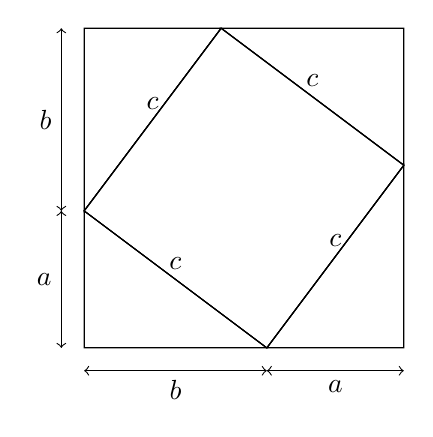
\begin{tikzpicture}[scale=0.58]
    \def\a{3}
    \def\b{4}

    % 大きな正方形
    \draw (0,0) rectangle (\a+\b,\a+\b);

    % 4つの直角三角形
    \draw (0,0) -- (\b,0) -- (0,\a) -- cycle;
    \draw (0,\a) -- node[midway,above] {$c$} (\b,0);

    \draw (\b,0) -- (\a+\b,0) -- (\a+\b,\b) -- cycle;
    \draw (\a+\b,\b) -- node[midway,above] {$c$} (\b,0);

    \draw (\a+\b,\b) -- (\a+\b,\a+\b) -- (\a,\a+\b) -- cycle;
    \draw (\a,\a+\b) -- node[midway,above] {$c$} (\a+\b,\b);

    \draw (\a,\a+\b) -- (0,\a+\b) -- (0,\a) -- cycle;
    \draw (0,\a) -- node[midway,above] {$c$} (\a,\a+\b);

    % 中央の正方形
    \draw (\b,0) -- (\a+\b,\b) -- (\a,\a+\b) -- (0,\a) -- cycle;

    % 寸法
    \draw[<->] (-0.5,0) -- (-0.5,\a) node[midway,left] {$a$};
    \draw[<->] (-0.5,\a) -- (-0.5,\a+\b) node[midway,left] {$b$};
    \draw[<->] (0,-0.5) -- (\b,-0.5) node[midway,below] {$b$};
    \draw[<->] (\b,-0.5) -- (\a+\b,-0.5) node[midway,below] {$a$};
  \end{tikzpicture}
\end{example}


\begin{mycolumn}
  証明を記述する際には，文末に$\square$や$\blacksquare$をかくことが一般的である．そのほかに``Q.E.D.''\footnote{``quod erat demonstrandum''の略で，ラテン語で「証明されるべきであったこと」という意味である．}などの表現も用いられる．
\end{mycolumn}

\phantomsection
\section{さまざまな証明法}

命題が真であることを示す方法にも，偽であることを示す方法にも，さまざまなものがある．代表的なものを挙げてみよう．

\begin{description}[descnext]
  \item[帰納法\index{きのうほう@帰納法}]
        たとえば数学的帰納法は，数学的な主張が自然数全体に対して成り立つことを示すための証明法である．
  \item[背理法\index{はいりほう@背理法}]
        「$P$が成り立たないと仮定すると矛盾が生じる」という論理的な構造を用いて証明を行う方法である．
  \item[直接証明\index{ちょくせつしょうめい@直接証明}]
        「$P$が成り立つことを示す」という形式で証明を行う方法である．
  \item[反例による反証\index{はんれい@反例}]
        全称命題「すべての$x$について$P(x)$が成り立つ」が\textbf{偽}であることを示すには，$P(x)$が成り立たない$x$，すなわち\emph{反例}をひとつ挙げれば十分である．
\end{description}

以下では，まず「$n \geqq 2$ を満たす任意の自然数について，$2^n > n$である」という命題を3通りのやり方で証明してみよう．

\phantomsection
\begin{example}{帰納法}{帰納法}
  \begin{enumerate}[(I)]
    \item $n=2$のとき，
          \[
            2^2 = 4 > 2
          \]

          となり，与えられた不等式は成立する．
    \item 自然数$k$を$k \geqq 2$を満たすように任意にとる．$2^k > k$ が成り立つと仮定する．このとき，
          \[
            2^{k+1} = 2 \cdot 2^k > 2k
          \]
          である．
          ここで，$k \geqq 2$であるから，$2k - (k + 1) = k - 1 \geqq 1$であるがゆえに，$2k > k + 1$である．

          したがって，

          \[
            2^{k+1} > 2k > k + 1
          \]
          である．
          ゆえに，$n=k+1$のときも$2^{k+1} > k + 1$である．
  \end{enumerate}

  以上の考察と数学的帰納法により，$2^n > n$ は $n \geqq 2$を満たすすべての自然数について成り立つ．これが証明すべきことであった．\qed
\end{example}

\phantomsection
\begin{example}{背理法}{背理法}
  $n \geqq 2$を満たす自然数で $2^n \leqq n$ となるものが存在すると仮定する．
  $2^n$ の正の約数の個数は，指数に $1$ を加えたものなので，$2^n$の正の約数の個数は $n + 1$ 個以上である．
  しかし，仮定より $2^n \leqq n$ なので，$2^n$ は $n$ 以下の数である．

  これは，$n$ 以下の数が $n + 1$ 個以上の正の約数を持つことを意味するが，これは矛盾である．

  したがって，先の仮定が誤りであるため，背理法によって$2^n > n$ が成り立つ．これが証明すべきことであった．\qed
\end{example}

\phantomsection
\begin{example}{直接証明}{直接証明}
  \[
    2^n = n \int_{1}^{2} x^{n-1} \, dx + 1
  \]
  となることはよい．さて，$x \in [1, 2]$ かつ $n \geqq 2$ なので，
  \[
    x^{n-1} \geqq x^{1} \geqq 1
  \]
  が成り立つ．したがって，
  \begin{align*}
    2^n & = n \int_{1}^{2} x^{n-1} \, dx + 1 \\
        & \geqq  n \int_{1}^{2} \, dx +1     \\
        & = n+1
  \end{align*}
  である．
  これと$n+1 >n$であることを併せると，$n \geqq 2$のとき$2^n > n$である．これが証明すべきことであった．\qed
\end{example}

最後に，反例による反証の例を見てみよう．全称命題は「すべての場合において成り立つ」ことを主張しているため，ひとつでも例外があれば命題全体が偽となる．したがって，命題が偽であることの証明としては，反例をひとつ示すだけで十分なのである．

\phantomsection
\begin{example}{反例による反証}{反例による反証}
  次の命題を考える：
  \[
    \forall n \in \mathbb{N}\, : \, \frac{n^3}{24} + 84 \geqq n^2
  \]
  この命題が成り立たないことを示すためには，ある$n$について不等式が成立しないことを示せばよい．実際に，$n = 15$のとき，
  \[
    \frac{15^3}{24} + 84 = \frac{3375}{24} + 84 = 140.625 + 84 = 224.625
  \]
  である．
  一方，
  \[
    15^2 = 225
  \]
  である．
  したがって，
  \[
    \frac{15^3}{24} + 84 = 224.625 < 225 = 15^2
  \]
  が成り立つ．
  このように，$n = 15$において不等式が成り立たないため，元の命題は偽であることがわかる．
\end{example}

また，全称命題が偽であることを証明する際には，「反例をどう見つけたか」ということは明記しない場合が多い．
たとえば\exref{反例による反証}の場合に$n=15$を見つけるには，微分法を用いて議論したりさまざまな方法があるが，そのような「反例を見つけるまでの過程」を説明する必要はなく，「$n=15$の場合に命題が成り立たないこと」のみを証明として書けばよい．

\phantomsection
\section{数学における存在と一意性}

ここまでで，証明とはなにか，そしてどのような証明法があるかを確認した．
本節では，数学的な主張そのものの論理構造に一歩踏み込み，「存在する」という主張と「ただひとつである」という主張について考える．
これらは単なる言い回しではなく，「数学では何を証明しなければならないのか」を決める骨格である．

\phantomsection
\subsection{存在}

数学の証明において，「存在\index{そんざい@存在}」は重要な概念である．といっても，あまりこのことを意識したことのない読者の方もいると思うので，この場を借りて具体例をもとに説明を試みることとする．

まず，以下に記す「最大値・最小値の定理」を考える：
\begin{quotation}
  $[a,b]$で連続な関数$f$に対して，$f$は$[a,b]$上で最大値と最小値を持つ．
\end{quotation}

「最大値・最小値が存在するなんて当たり前だ」と思われる読者もいるかもしれない．しかし，本当にそれは自明なのか．
実際には，関数の連続性や区間の閉有界性といった条件が揃って初めて，最大値や最小値の「存在」を保証できる．この定理を証明するにあたっては，厳密な数学的議論が必要となる．

「存在」の重要性がわかる例として，「極限値の存在」に関する命題を以下で考えてみよう：

\begin{prop}{}{}
  以下のような漸化式で定められた数列$(x_n)_{n \in \mathbb{N}}$を考える：
  \[
    \begin{cases}
      x_1 =0 , \\
      x_{n+1}= \sqrt{x_n+2}
    \end{cases}
  \]
  このとき，$(x_n)_{n \in \mathbb{N}}$は収束し，極限値は次のようになる：
  \[
    \lim_{n \to \infty} x_n =2
  \]
  が成り立つ．
\end{prop}

\begin{tleftbar}
  \begin{proof}
    いくつかの補題を確認しつつ示す．
    \begin{lemma}{}{}
      任意の$n \in \mathbb{N}$に対して，以下の不等式が成り立つ：
      \[
        x_n \leqq x_{n+1} < 2
      \]
    \end{lemma}
      \begin{proof}
        数学的帰納法により，$x_n \leqq x_{n+1} < 2$を示す．
        \begin{enumerate}[(I)]
          \item \mbox{} \\ \label{proof:存在1}
                $n=1$のとき，$ x_1 =0$，$x_2= \sqrt{0+2}=\sqrt{2}$なので，$ 0 \leqq \sqrt{2} < 2$により，
                $x_1 \leqq x_2 < 2$である．
          \item \mbox{} \\ \label{proof:存在2}
                $k \in \mathbb{N}$を任意にとり，$x_k \leqq x_{k+1} < 2$であると仮定する．

                このとき，$x_{k+1} < 2$により$ x_{k+1}+2 < 4$なので，以下の式が成り立つ：
                \[
                  x_{k+2}=\sqrt{x_{k+1} + 2} < 2
                \]

                また，$x_k \leqq x_{k+1}$により，$x_k +2  \leqq x_{k+1}+2$であるから，
                \[
                  x_{k+1}= \sqrt{x_k +2} \leqq \sqrt{x_{k+1}+2}=x_{k+2}
                \]
                が成り立つ．
                よって，$n=k+1$の場合にも成り立つ．
        \end{enumerate}
        以上\ref{proof:存在1}，\ref{proof:存在2}により，任意の$n \in \mathbb{N}$について，以下の不等式が成り立つ：
        \[
          x_n \leqq x_{n+1} < 2.
        \]
      \end{proof}
    \begin{lemma}{}{}
      $(x_n)_{n \in \mathbb{N}}$は$ 0<  x \leqq 2$なる極限$x$に収束する．
    \end{lemma}
      \begin{proof}
        先の補題により，任意の$n \in \mathbb{N}$について，$ x_n \leqq x_{n+1} <2$なので，
        数列$(x_n)_{n \in \mathbb{N}}$は単調に増加し，上に有界である．

        よって
        \[
          x \coloneqq \sup \{ x_n \mid n \in \mathbb{N} \}
        \]
        が存在し，$x \leqq  2$である．

        $ x>0$は明らかである．これが証明すべきことであった．
      \end{proof}

    ここまでで，$(x_n)_{n \in \mathbb{N}}$の極限値の存在が確認されたので，先の漸化式について，
    \[
      x=\sqrt{x+2}
    \]
    とする．これを解くと$ x= -1,2$であるが，$x>0$により$x=2$である．

    以上の考察により，数列$(x_n)_{n \in \mathbb{N}}$は収束し，
    \[
      \lim_{n \to \infty} x_n =2
    \]
    が成り立つ．これが証明すべきことであった．
  \end{proof}
\end{tleftbar}

ここまで考察して，ようやく数列$(x_n)_{n \in \mathbb{N}}$が収束することを確認できた．
この例では「極限値の存在」を確認する意味がわからない読者もいるかもしれないので，もうひとつ例を挙げよう．


以下のような漸化式で定められた数列$(y_n)_{n \in \mathbb{N}}$を考える：
\[
  \begin{cases}
    y_1 =1 , \\
    y_{n+1}= 2y_n +2
  \end{cases}
\]
この数列の極限値が存在すると仮定して，それを$y$とおこう．
\begin{tleftbar}
  与えられた漸化式により，
  \begin{align*}
     & y = 2y +2,           \\
     & \therefore ~ y = -2.
  \end{align*}
  しかし，
  \[
    \lim_{n \to \infty} y_n = \infty
  \]
  なので，$y=-2$は誤りである．
\end{tleftbar}

このように，数列の極限が存在することを確認しないと，誤った結論に到達することがある．この例からわかるように，存在を確認することは重要なことなのである．


\phantomsection
\subsection{一意性}

\begin{wrapfigure}[10]{r}{0.425\textwidth}
  %\centering
  \begin{tikzpicture}[scale=0.78]
    \begin{axis}[
        axis lines=middle,
        xmin=-1.2, xmax=1.2,
        ymin=-1.5, ymax=1.5,
        xtick=\empty, ytick=\empty, % 目盛を消す
        xlabel={}, ylabel={},       % ラベルを消す
        samples=200,
        domain=-1.2:1.2,
        width=10cm,
        height=8cm,
      ]
      % 関数 f(x) = x^3 のグラフ
      \addplot [dblue, thick] {x^3};

      % 点 (-1, -1) と (1, 1) を結ぶ割線
      \addplot [dred, thick] coordinates {(-1, -1) (1, 1)};

      % 平均値の定理を満たす点 x = -1/√3 の接線
      \def\xone{-1/sqrt(3)}
      \def\yone{(\xone)^3}
      \addplot [dgreen, dashed] {1*(x - \xone) + \yone};

      % 平均値の定理を満たす点 x = 1/√3 の接線
      \def\xtwo{1/sqrt(3)}
      \def\ytwo{(\xtwo)^3}
      \addplot [dgreen, dashed] {1*(x - \xtwo) + \ytwo};

      % 重要な点をマーク
      \addplot [only marks, mark=*, mark options={fill=black}] coordinates {(\xone, \yone) (\xtwo, \ytwo)};
      \addplot [only marks, mark=*, mark options={fill=dred}] coordinates {(-1, -1) (1, 1)}; % 赤い丸に変更
    \end{axis}
  \end{tikzpicture}
\end{wrapfigure}

読者の中には線型代数の講義で「逆行列の一意性」などに触れた方もいると思われる．線型代数以外の分野でも，数学の学習を進める際に，「一意性\index{いちいせい@一意性}」が重要である場面は多い．なぜ「一意性」が重要であるのか，ひとつ例を挙げて考えてみることにしよう．

微分積分の講義で習う定理に「平均値の定理」というものがある．
その主張は
\begin{quotation}
  $[a,b]$で連続，$(a,b)$で微分可能な関数$f$に対して，
  \[
    \frac{f(b)-f(a)}{b-a}=f'(c)
  \]
  を満たす$ c \in (a,b)$が存在する．
\end{quotation}

というものである．証明はのちに述べるとして，この定理の主張を少し変更してみよう：

\begin{quotation}
  $[a,b]$で連続，$(a,b)$で微分可能な関数$f$に対して，
  \[
    \frac{f(b)-f(a)}{b-a}=f'(c)
  \]
  を満たす$ c \in (a,b)$がただひとつ存在する．
\end{quotation}


ここで「$c \in (a,b)$が存在する」という主張を「$c \in (a,b)$がただひとつ存在する」というより強い主張に変更した．この主張は偽である．このことが問題になる状況を挙げよう．
$f(x)=x^3$という関数を考える．この関数は$[-1,1]$で連続，$(-1,1)$で微分可能である．
このとき，図のように，条件を満たす$c \in (-1,1)$は複数存在するので，「ただひとつ存在する」という主張は偽である．
さらに言えば，2本より多くこのような接線を引ける場合もある\footnote{各自で確認してみてほしい．}．

このことから，安易に「ただひとつ存在する」などと強い主張をすることは避けるべきであることがわかる．このことは平均値の定理に限らず，中間値の定理なども同様である．

\phantomsection
\subsection{存在と一意性の違い}

ここまでの考察からわかるように，「存在する」という主張と「ただひとつである」という主張は，別々に考える必要がある．
とくに，一意性を示すことは，それ自体では存在を保証しない．
典型的な例を整理すると，次のようになる．

\begin{center}
  \begin{tabular}{|c|p{9.5cm}|}
    \hline
    \textbf{状況} & \textbf{例} \\ \hline

    存在し，一意である
    &
    正則行列\footnote{逆行列を持つ正方行列のことを正則行列という．}の逆行列，
    方程式$x^3 = 8$の実数解など．
    \\ \hline

    存在するが，一意ではない
    &
    方程式$x^2 = 4$の実数解など．
    また，平均値の定理によって存在が保証される$c$も，一般には一意とは限らない．
    \\ \hline

    存在しない
    &
    方程式$x^2 = -1$の実数解など．
    \\ \hline

    一意性だけが示されている
    &
    存在するかどうかとは別に，
    「もし存在するなら，それはただひとつである」とだけ示されている場合である．
    \prref{逆行列の一意性}がこの形の主張である．
    \\ \hline
  \end{tabular}
\end{center}

したがって，ある対象が「ただひとつ存在する」ことを示すには，
\textbf{存在性}と\textbf{一意性}の両方を示さなければならない．

\begin{remark}[「存在」と「一意性」は別の課題]
  とくに，「一意性だけが示されている」場合に注意しよう．
  \prref{逆行列の一意性}をあらためて見返すと，
  「存在するとすれば」とあるように，この命題は逆行列の存在を一切主張していない．
  実際，逆行列を持たない正方行列は存在する\footnote{たとえば零行列．}．
  このように，一意性の証明は存在の証明と切り離して，ときには存在の証明よりも先に行うことができる．
  「存在」と「一意性」は，証明においても別々に扱われるべきふたつの課題なのである．
\end{remark}

% NOTE: この部は執筆中（今後，節を追記する可能性あり）

\phantomsection
\part{集合}

\begin{abstract}
この章では，現代数学の基礎をなす「集合」を導入する．まず集合と元を定義し，集合の相等・部分集合・真部分集合といった基本概念を確認する．次に，$\mathbb{N}$，$\mathbb{Z}$，$\mathbb{Q}$，$\mathbb{R}$，$\mathbb{C}$ などのよく使う集合の記号と，外延的記法・内包的記法という集合の表記法を整理する．最後に，共通部分・和集合・差集合・補集合といった集合の演算を定義し，交換法則・分配律・ド・モルガンの法則などの基本性質を証明しよう．
\end{abstract}

\phantomsection
\section{集合の定義と表記法}

\phantomsection
\subsection{集合の定義}

現代数学の基礎をなす概念に「集合」や「写像」がある．まず「集合」からみていこう．
\phantomsection
\begin{definition}{集合}{集合}
  もののあつまりを\emph{集合}\index{しゅうごう@集合}という\footnote{公理的集合論の立場では，集合とは「無定義語」であるが，ここで詳しくは触れない．}．集合を構成するものを\emph{元}\index{げん@元}または\emph{要素}\index{ようそ@要素}といい，集合$A$の元が$a$であることを$a \in A$，$A \ni a$などと表す．
\end{definition}

\begin{remark}[集合の表記に関する注意]
  集合について，いくつか注意しておこう．
  \begin{itemize}
    \item 要素の順序は問わない．たとえば，$\{1,2,3\}=\{3,2,1\}$である．
    \item 同じ要素を重複して書いても同じ集合を表す．たとえば，$\{1,1,2,2,2,3\}=\{1,2,3\}$である．
    \item 異なる種類のものを要素にすることもできる．たとえば，$\{4,\{3\}\}$は数$4$と集合$\{3\}$を要素に持つ．
  \end{itemize}
\end{remark}

次に，ある集合の要素の一部または全部からなる集合を考える．これを\emph{部分集合}という．まずはその定義を確認し，具体例はのちほど紹介する．

\begin{definition}{集合の相等}{集合の相等}
  集合$A$，$B$のすべての要素が一致しているとき，$A$と$B$は\emph{相等}\index{そうとう@相等}であるといい，これを
  \[
    A = B
  \]
  と表す．

  また，集合$A$と$B$が相等でないとき，
  \[
    A \ne B
  \]
  と表す．
\end{definition}

\begin{remark}[相等を考える意義]
  \deref{集合の相等}を考える意義がぴんとこない読者もいるかもしれない．
  だが，たとえば$\pi$，$\int_{0}^{1} \frac{4}{1+x^2} \, dx$，$4 \sum_{n=0}^{\infty} \frac{(-1)^n}{2n+1}$は異なる表現であるが，すべて円周率を表している．
  このような例からわかるように，「相等」を考えることは数学的な主張を正確に表現するために重要なことなのだ．
\end{remark}

\phantomsection
\begin{definition}{部分集合}{部分集合}
  集合$A$の要素がすべて集合$B$の要素でもあるとき，$A$は$B$の\emph{部分集合}\index{ぶぶんしゅうごう@部分集合}であるといい，これを
  \[
    A \subset B,\quad B \supset A
  \]
  などと表す\footnote{このことを$ A \subseteq B$，$B \supseteq A$とかくこともある．一般に，$A \subset B$，$ B \supset A$と書いた場合には$A=B$の場合を含んで意味をとる．}．
\end{definition}

\begin{definition}{真部分集合}{真部分集合}
  集合$A$の要素がすべて集合$B$の要素であり，なおかつ$A \ne B$であるとき，$A$は$B$の\emph{真部分集合}\index{しんぶぶんしゅうごう@真部分集合}であるといい，これを
  \[
    A \subsetneq B,\quad B \supsetneq A
  \]
  などと表す．
\end{definition}

集合の相等は，部分集合の言葉を用いて次のように特徴づけられる．

\phantomsection
\begin{prop}{相等と相互包含}{相等と相互包含}
  集合$A$，$B$に対して，
  \[
    A = B
    \lequiv
    (A \subset B) \land (B \subset A)
  \]
  である．また，量化子を用いれば，
  \[
    A = B
    \lequiv
    \lall{x} \lst ( x \in A \lequiv x \in B )
  \]
  と表すこともできる．
\end{prop}

\begin{tleftbar}
  \begin{proof}
    \deref{集合の相等}より，$A = B$とは$A$と$B$のすべての要素が一致すること，すなわち「任意の$x$について，$x \in A$と$x \in B$の真偽が一致する」ことである．一方，$A \subset B$は「任意の$x$について，$x \in A$ならば$x \in B$」を，$B \subset A$は「任意の$x$について，$x \in B$ならば$x \in A$」を意味する．同値の等価表現$P \lequiv Q \equiv (P \limp Q) \land (Q \limp P)$により，両者は一致する．これが証明すべきことであった．
  \end{proof}
\end{tleftbar}

この命題は，集合の等式$A = B$を証明するための\textbf{標準的な方法}を与えている．すなわち，$A \subset B$と$B \subset A$の\textbf{両方向の包含}をそれぞれ示せばよい．のちに集合の分配律を証明する際にも，実際にこの方法を用いる．

\phantomsection
\subsection{集合の表記}

集合を表す方法には，おもに次の2つがある．

\begin{description}
  \item[外延的記法\index{がいえんてききほう@外延的記法}（列挙形式）]
        $\{a,b,c\}$のように，要素を列挙して表す．
  \item[内包的記法\index{ないほうてききほう@内包的記法}（条件形式）]
        $\{x\in\mathbb{N}\mid x\leqq5\}$のように，
        要素が満たす条件を用いて表す．
\end{description}

\begin{example}{集合の表記}{集合の表記}
  集合は，外延的記法と内包的記法のどちらを用いても表すことができる．
  たとえば，次の等式が成り立つ．
  \begin{align*}
    \{1,2,3\}
      &=
      \{n\in\mathbb{N}\mid n^2-4n+3\leqq0\},\\
    \{-2,-1,0,1,2\}
      &=
      \{n\in\mathbb{Z}\mid n^2\leqq4\},\\
    \{2,4,6,8,\dots\}
      &=
      \{2n\mid n\in\mathbb{N}\},\\
    \{1,4,9,16,25,\dots\}
      &=
      \{n^2\mid n\in\mathbb{N}\},\\
      \{-1,1\} &= \{x\in\mathbb{R}\mid x^{2026}=1\}.
  \end{align*}
\end{example}

また数学では，よく使われる集合に固有の記号を用いることがある．

\begin{reviewbox}[数の集合]
  \small
  \begin{tabular}{@{}p{14\zw}@{\hspace{1.5\zw}}l@{}}
    自然数（natural numbers）&
    $\mathbb{N} = \{1,2,3,\ldots\}$\footnotemark\\[0.35\baselineskip]

    整数（integers）&
    $\mathbb{Z} = \{\ldots,-2,-1,0,1,2,\ldots\}$\\[0.35\baselineskip]

    有理数（rational numbers）&
    $\mathbb{Q} = \left\{ \frac{a}{b} \relmiddle| a \in \mathbb{Z},\ b \in \mathbb{N} \right\}$\\[0.35\baselineskip]

    実数（real numbers）&
    $\mathbb{R}$\\[0.35\baselineskip]

    複素数（complex numbers）&
    $\mathbb{C} = \{ a + bi \mid a,b \in \mathbb{R} \}$
  \end{tabular}
  \footnotetext{自然数に$0$を含める流儀もあるが，本書では自然数に$0$を含めないものとする．}
\end{reviewbox}

$\mathbb{N}$，$\mathbb{R}$，$\mathbb{C}$は，それぞれ natural number，real number，complex number に由来する記号である．
また，$\mathbb{Z}$はドイツ語の Zahl（数）に，$\mathbb{Q}$は quotient（商）に由来する．
なお，$\mathbb{C}$の表記に現れる$i$は，$i^2 = -1$を満たす\emph{虚数単位}である．$i$は内包的記法の中で動く変数ではなく，あらかじめ固定された定数であることに注意したい．


$x$がどの集合の中を動くかは，文脈により省略されることがある．たとえば，以下のような問題があったとする．
\begin{quotation}
  方程式
  \[
    x^2 + 1 = 0
  \]
  を解け．
\end{quotation}
この問題では，$x$がどの集合の中を動くかが明記されていない．
もし$x \in \mathbb{R}$の範囲で解を探すなら，任意の実数$x$に対して$x^2 + 1 \geqq 1 > 0$なので，解は存在しない．
一方，$x \in \mathbb{C}$の範囲で解を探すなら，解は$x = \pm i$である．
このように，「方程式を解く」という問題の答えは，\textbf{どの集合の中で解を探しているか}によって変わる．
$x$が動く集合は，文脈から読み取れたり明記されていたりする場合が多いが，答えが変わりうる以上，つねに意識しておきたいことがらである．

数の集合以外にも，特定の集合を表すために固有の記号を用いることがある．

\phantomsection
\begin{definition}{空集合}{空集合}
  要素をひとつも持たない集合を\emph{空集合}\index{くうしゅうごう@空集合}といい，
  \[
    \varnothing
  \]
  で表す．
\end{definition}

空集合は$\emptyset$と表記することもある\footnote{空集合をギリシャ文字の$\phi$で表記するのは誤りである．空集合の記号$\varnothing$はAndré Weilによって導入されたもので，ノルウェー語やデンマーク語などで用いられる文字Øに着想を得ている．}．

\phantomsection
\begin{example}{空集合の例}{空集合の例}
  空集合は，外延的記法では
  \[
    \{\}
  \]
  と表される．一方，内包的記法では，たとえば
  \[
    \{x \in \mathbb{R} \mid x^2=-1\},
    \qquad
    \{n \in \mathbb{N} \mid n<0\},
    \qquad
    \{x \in \mathbb{R} \mid x<x\}
  \]
  は，いずれも条件を満たす要素をひとつも持たないため，空集合である．
  したがって，
  \[
    \{\}
    =
    \{x \in \mathbb{R} \mid x^2=-1\}
    =
    \{n \in \mathbb{N} \mid n<0\}
    =
    \{x \in \mathbb{R} \mid x<x\}
    =
    \varnothing
  \]
  である．
\end{example}

\begin{remark}[空集合に関する注意]
  空集合について，いくつか注意しておこう．
  \begin{itemize}
    \item 空集合は要素をひとつも持たないので，どのような$x$に対しても，$x \in \varnothing$は\textbf{常に偽}である．いいかえれば，任意の$x$に対して$x \notin \varnothing$が成り立つ．
    \item 集合
          \[
            \{\varnothing\}
          \]
          は空集合$\varnothing$をひとつの要素として持つ集合であり，空集合ではない．
    \item 空集合の要素の個数は$0$である．一般に，有限集合$A$の要素の個数を$|A|$や$n(A)$と表すことがあり，この記法を用いれば
          \[
            |\varnothing| = 0, \qquad |\{\varnothing\}| = 1
          \]
          である．
  \end{itemize}
\end{remark}

\phantomsection
\begin{example}{所属関係の例}{所属関係の例}
  \[
    x \in \mathbb{Q}
  \]
  とかくことで，$x$は有理数であることを表す．
\end{example}

\phantomsection
\begin{example}{部分集合の例}{部分集合の例}
  \[
    \mathbb{R} \subset \mathbb{C}
  \]
  である．つまり，実数全体の集合は複素数全体の集合の部分集合である．
\end{example}

\phantomsection
\begin{prop}{空集合は任意の集合の部分集合}{空集合は任意の集合の部分集合}
  $A$を任意の集合とするとき，
  \[
    \varnothing \subset A
  \]
  である．つまり，空集合はすべての集合の部分集合である．
\end{prop}

\begin{tleftbar}
  \begin{proof}
    部分集合の定義（\deref{部分集合}）より，$\varnothing \subset A$を示すには，
    \begin{quotation}
      任意の$x$に対して，$x \in \varnothing$ならば$x \in A$である
    \end{quotation}
    ことを示せばよい．ところが，空集合は要素をひとつも持たないので，$x \in \varnothing$を満たす$x$は存在しない．すなわち，仮定「$x \in \varnothing$」はどのような$x$に対しても偽である．仮定が偽である命題は結論によらず真であるから\footnote{このように，仮定を満たすものが存在しないために無条件で真となることを，\emph{空虚な真}（vacuous truth）ということがある．}，「$x \in \varnothing$ならば$x \in A$」は任意の$x$に対して真である．よって$\varnothing \subset A$が成り立つ．
  \end{proof}
\end{tleftbar}

\begin{remark}[背理法による見方]
  次のように考えることもできる．もし$\varnothing \subset A$が成り立たないとすると，「$\varnothing$の要素であって$A$に属さないもの」が少なくともひとつ存在しなければならない．しかし，$\varnothing$はそもそも要素を持たないので，そのような要素は存在しえない．よって$\varnothing \subset A$である．
\end{remark}

集合を要素とする集合の重要な例として，べき集合がある．

\phantomsection
\begin{definition}{べき集合}{べき集合}
  集合$A$に対して，$A$の部分集合全体からなる集合
  \[
    \mathcal{P}(A) \coloneqq \{ B \mid B \subset A \}
  \]
  を$A$の\emph{べき集合}\index{べきしゅうごう@べき集合}という．
\end{definition}

\prref{空集合は任意の集合の部分集合}により，つねに$\varnothing \in \mathcal{P}(A)$である．また，$A \subset A$なので$A \in \mathcal{P}(A)$である．

\phantomsection
\begin{example}{べき集合}{べき集合}
  $A=\{ 1, 2\}$とすると，
  \[
    \mathcal{P}(A) = \{ \varnothing, \{1\}, \{2\}, \{1, 2\}\}
  \]
  である．
\end{example}



\phantomsection
\section{集合の演算}

\subsection{共通部分・和集合・差集合・補集合}
集合に対して，以下のような演算を定義することができる．

\phantomsection
\begin{definition}{共通部分・和集合・差集合・補集合}{共通部分・和集合・差集合・補集合}
  $A$と$B$を集合とするとき，以下の定義をする．
  \begin{description}
    \item[共通部分\index{きょうつうぶぶん@共通部分}]\mbox{}\\
          $A$と$B$の両方に属する要素全体の集合を$A \cap B$と表す．これを``$A$ intersection $B$''と読む．
    \item[和集合\index{わしゅうごう@和集合}]\mbox{}\\
          $A$または$B$のいずれかに属する要素全体の集合を$A \cup B$と表す．これを``$A$ union $B$''と読む．
    \item[差集合\index{さしゅうごう@差集合}]\mbox{}\\
          $A$の要素で$B$に属さないもの全体の集合を$A \setminus B$と表す．
    \item[補集合\index{ほしゅうごう@補集合}]\mbox{}\\
          全体集合$X$\footnote{考察の対象すべてを含む集合をあらかじめひとつ固定して考えるとき，その集合を\emph{全体集合}\index{ぜんたいしゅうごう@全体集合}という．}とその部分集合$A \subset X$に対して，$A^c \coloneqq X \setminus A$を$A$の補集合という．これを``$A$ complement''と読む．
  \end{description}
\end{definition}

\begin{remark}[論理記号による言い換え]
  集合の演算は，\partref{論理}で学んだ論理記号を用いて次のように言い換えられる：
  \begin{align*}
    x \in A \cap B & \lequiv (x \in A) \land (x \in B), \\
    x \in A \cup B & \lequiv (x \in A) \lor (x \in B), \\
    x \in A \setminus B & \lequiv (x \in A) \land \lnot (x \in B), \\
    x \in A^c & \lequiv \lnot (x \in A) \qquad (x \in X)
  \end{align*}
  すなわち，$\cap$は$\land$に，$\cup$は$\lor$に，補集合は$\lnot$に対応している．また，部分集合についても
  \[
    A \subset B \lequiv \lall{x} \lst ( x \in A \limp x \in B )
  \]
  である．この対応により，命題論理の法則から集合の法則を導くことができる（のちのド・モルガンの法則の証明で実際に用いる）．
\end{remark}


\begin{figure}[ht]
  \centering
  % --- ベン図の共通設定 ---
  \tikzset{
    venn frame/.style={
      draw=black!75,
      line width=0.7pt
    },
    venn circle/.style={
      draw=black!85,
      line width=0.8pt
    },
    venn fill/.style={
      fill=magenta!15
    },
    venn label/.style={
      font=\small
    }
  }
  % --- 共通部分 ---
  \begin{minipage}{0.45\linewidth}
    \centering
    \begin{tikzpicture}[scale=0.9]
      % 塗り
      \begin{scope}
        \clip (2.2,2) circle (1.45);
        \fill[venn fill] (3.8,2) circle (1.45);
      \end{scope}

      % 輪郭
      \draw[venn frame] (0,0) rectangle (6,4);
      \draw[venn circle] (2.2,2) circle (1.45);
      \draw[venn circle] (3.8,2) circle (1.45);

      % ラベル
      \node[venn label] at (1.35,2.9) {$A$};
      \node[venn label] at (4.65,2.9) {$B$};
      \node[venn label, anchor=north east] at (5.85,3.85) {$X$};
    \end{tikzpicture}
    \caption{共通部分 $A \cap B$}
  \end{minipage}
  \hfill
  % --- 和集合 ---
  \begin{minipage}{0.45\linewidth}
    \centering
    \begin{tikzpicture}[scale=0.9]
      % 塗り
      \fill[venn fill] (2.2,2) circle (1.45);
      \fill[venn fill] (3.8,2) circle (1.45);

      % 輪郭
      \draw[venn frame] (0,0) rectangle (6,4);
      \draw[venn circle] (2.2,2) circle (1.45);
      \draw[venn circle] (3.8,2) circle (1.45);

      % ラベル
      \node[venn label] at (1.35,2.9) {$A$};
      \node[venn label] at (4.65,2.9) {$B$};
      \node[venn label, anchor=north east] at (5.85,3.85) {$X$};
    \end{tikzpicture}
    \caption{和集合 $A \cup B$}
  \end{minipage}

  \vspace{3mm}

  % --- 差集合 ---
  \begin{minipage}{0.45\linewidth}
    \centering
    \begin{tikzpicture}[scale=0.9]
      % A を塗る
      \fill[venn fill] (2.2,2) circle (1.45);

      % A \cap B の部分を白く戻す
      \begin{scope}
        \clip (2.2,2) circle (1.45);
        \fill[white] (3.8,2) circle (1.45);
      \end{scope}

      % 輪郭
      \draw[venn frame] (0,0) rectangle (6,4);
      \draw[venn circle] (2.2,2) circle (1.45);
      \draw[venn circle] (3.8,2) circle (1.45);

      % ラベル
      \node[venn label] at (1.35,2.9) {$A$};
      \node[venn label] at (4.65,2.9) {$B$};
      \node[venn label, anchor=north east] at (5.85,3.85) {$X$};
    \end{tikzpicture}
    \caption{差集合 $A \setminus B$}
  \end{minipage}
  \hfill
  % --- 補集合 ---
  \begin{minipage}{0.45\linewidth}
    \centering
    \begin{tikzpicture}[scale=0.9]
      % X 全体を塗る
      \fill[venn fill] (0,0) rectangle (6,4);

      % A を白く抜く
      \fill[white] (2.2,2) circle (1.45);

      % 輪郭
      \draw[venn frame] (0,0) rectangle (6,4);
      \draw[venn circle] (2.2,2) circle (1.45);

      % ラベル
      \node[venn label] at (1.35,2.9) {$A$};
      \node[venn label, anchor=north east] at (5.85,3.85) {$X$};
    \end{tikzpicture}
    \caption{補集合 $A^c$}
  \end{minipage}
\end{figure}


\phantomsection
\begin{example}{集合}{集合}
  たとえば，$A = \{1, 2, 3\}$，$B = \{3, 4, 5\}$とすると，
  \begin{itemize*}
    \item $A \cap B = \{3\}$
    \item $A \cup B = \{1, 2, 3, 4, 5\}$
    \item $A \setminus B = \{1, 2\}$
    \item $X=\{1,2,3,4,5\}$とすると，$A^c = \{4, 5\}$
  \end{itemize*}
\end{example}

\begin{prop}{集合の交換法則}{集合の交換法則}
  $A$，$B$を集合とするとき，
  \[
    A \cap B = B \cap A , \quad A \cup B = B \cup A
  \]
  である．
\end{prop}

\begin{tleftbar}
  \begin{proof}
    共通部分および和集合の定義から従う．
  \end{proof}
\end{tleftbar}

\begin{remark}[交換法則を考える意義]
  ここで「なぜ交換法則を考えるのか」という疑問が生じるかもしれない．当たり前に成り立つことだと思える読者もいるかもしれないが，よく考えてみると「実数の減法」や「関数（写像）の合成」，「行列の積」など，
  数学において一般に交換法則が成り立たないものは数多く存在する．集合に対して交換法則を考える意義はそこにあるのである．
\end{remark}

\phantomsection
\begin{prop}{空集合との演算}{空集合との演算}
  $A$を任意の集合とするとき，
  \[
    A \cup \varnothing = A, \quad A \cap \varnothing = \varnothing
  \]
  である．
\end{prop}

\begin{tleftbar}
  \begin{proof}
    まず$A \cup \varnothing = A$を示す．$x \in A \cup \varnothing$とすると，$x \in A$または$x \in \varnothing$である．$x \in \varnothing$を満たす$x$は存在しないので，$x \in A$でなければならない．よって$A \cup \varnothing \subset A$である．逆に，$x \in A$ならば和集合の定義から$x \in A \cup \varnothing$なので，$A \subset A \cup \varnothing$である．以上より$A \cup \varnothing = A$が成り立つ．

    次に$A \cap \varnothing = \varnothing$を示す．$x \in A \cap \varnothing$とすると，特に$x \in \varnothing$であるが，そのような$x$は存在しない．すなわち$A \cap \varnothing$は要素をひとつも持たないので，$A \cap \varnothing = \varnothing$である．
  \end{proof}
\end{tleftbar}

\begin{remark}[空集合と差集合・直積]
  差集合についても，
  \[
    A \setminus \varnothing = A, \quad \varnothing \setminus A = \varnothing
  \]
  が成り立つ．これは差集合の定義から直ちに確かめられる．

  また，集合$A$，$B$に対して，$A$の要素と$B$の要素の順序対$(a,b)$全体の集合を\emph{直積}$A \times B$という（詳しくは\partref{写像}で定義する）．直積についても，
  \[
    A \times \varnothing = \varnothing, \quad \varnothing \times A = \varnothing
  \]
  が成り立つ．たとえば$(a, b) \in A \times \varnothing$となる順序対が存在するとすれば，$b \in \varnothing$でなければならないが，そのような$b$は存在しないからである．
\end{remark}

\subsection{集合の分配律}

\phantomsection
\begin{prop}{集合の分配律}{集合の分配律}
  $A$，$B$，$C$を集合とするとき，
  \begin{align*}
    A \cap ( B \cup C) & = (A \cap B) \cup (A \cap C), \\
    A \cup ( B \cap C) & = (A \cup B) \cap (A \cup C)
  \end{align*}
\end{prop}

\begin{tleftbar}
  \begin{proof}
    まず，
    \[
      A \cap (B \cup C) \subset (A \cap B) \cup (A \cap C)
    \]
    を示す：

    $x \in A \cap (B \cup C)$ とすると，$x$ は $A$ に属し，かつ $B \cup C$ に属する．
    すると $x \in B \cup C$ なので，$x \in B$ または $x \in C$ のいずれかが成り立つ．
    \begin{itemize}
      \item もし $x \in B$ であれば，$x$ は $A$ に属し $B$ にも属するので，$x \in A \cap B$ となる．よって $x \in (A \cap B) \cup (A \cap C)$ が従う．
      \item もし $x \in C$ であれば，$x$ は $A$ に属し $C$ にも属するので，$x \in A \cap C$ となる．よって $x \in (A \cap B) \cup (A \cap C)$ が従う．
    \end{itemize}
    いずれの場合でも $x \in (A \cap B) \cup (A \cap C)$ となるので，
    \[
      A \cap (B \cup C) \subset (A \cap B) \cup (A \cap C)
    \]
    が示された．

    次に，
    \[
      (A \cap B) \cup (A \cap C) \subset A \cap (B \cup C)
    \]
    を示す：

    $x \in (A \cap B) \cup (A \cap C)$ とすると，$x \in A \cap B$ または $x \in A \cap C$ のいずれかが成り立つ．
    \begin{itemize}
      \item もし $x \in A \cap B$ であれば，$x$ は $A$ に属し，かつ $B$ に属する．すると $B \subset B \cup C$ だから $x \in B \cup C$ でもある．よって $x \in A \cap (B \cup C)$ が成り立つ．
      \item もし $x \in A \cap C$ であれば，$x$ は $A$ に属し，かつ $C$ に属する．すると $C \subset B \cup C$ だから $x \in B \cup C$ でもある．よって $x \in A \cap (B \cup C)$ が成り立つ．
    \end{itemize}
    いずれの場合でも $x \in A \cap (B \cup C)$ となるので，
    \[
      (A \cap B) \cup (A \cap C) \subset A \cap (B \cup C)
    \]
    が示された．

    以上の2つの包含関係から，
    \[
      A \cap (B \cup C) =(A \cap B) \cup (A \cap C)
    \]
    が成り立つ．後半の等式も同様に示される．これが証明すべきことであった．
  \end{proof}
\end{tleftbar}

\subsection{集合のさまざまな法則}

\phantomsection
\begin{prop}{べき等律・全体集合との演算・補集合の性質}{べき等律・全体集合との演算・補集合の性質}
  $X$を全体集合，$A \subset X$とするとき，次が成り立つ：
  \begin{align*}
    & A \cup A = A, && A \cap A = A, \\
    & A \cup X = X, && A \cap X = A, \\
    & A \cup A^c = X, && A \cap A^c = \varnothing, \\
    & (A^c)^c = A
  \end{align*}
\end{prop}

\begin{tleftbar}
  \begin{proof}
    いずれも定義から確かめられる．例として$(A^c)^c = A$を示す．$x \in X$に対して，
    \[
      x \in (A^c)^c
      \lequiv \lnot ( x \in A^c )
      \lequiv \lnot \lnot ( x \in A )
      \lequiv x \in A
    \]
    である（最後の同値は二重否定$\lnot \lnot P \equiv P$による）．よって$(A^c)^c = A$である．残りも同様に示される．
  \end{proof}
\end{tleftbar}

\phantomsection
\begin{prop}{集合のド・モルガンの法則}{集合のド・モルガンの法則}
  $X$を全体集合，$A, B \subset X$とするとき，
  \[
    (A \cup B)^c = A^c \cap B^c,
    \qquad
    (A \cap B)^c = A^c \cup B^c
  \]
  が成り立つ．
\end{prop}

\begin{tleftbar}
  \begin{proof}
    前半を示す．$x \in X$に対して，
    \begin{align*}
      x \in (A \cup B)^c
      & \lequiv \lnot ( x \in A \cup B ) \\
      & \lequiv \lnot \bigl( (x \in A) \lor (x \in B) \bigr) \\
      & \lequiv \lnot (x \in A) \land \lnot (x \in B) \\
      & \lequiv x \in A^c \cap B^c
    \end{align*}
    である．途中，3つ目の同値で命題論理のド・モルガンの法則$\lnot (P \lor Q) \equiv \lnot P \land \lnot Q$を用いた．\prref{相等と相互包含}の論理式による特徴づけにより，$(A \cup B)^c = A^c \cap B^c$である．後半も同様に示される．これが証明すべきことであった．
  \end{proof}
\end{tleftbar}

\begin{remark}[論理の法則と集合の法則]
  この証明からわかるように，集合のド・モルガンの法則は，命題論理のド・モルガンの法則を$P = (x \in A)$，$Q = (x \in B)$として集合の言葉に翻訳したものにほかならない．同様に，集合の交換法則・結合律・分配律も，命題論理の対応する法則から導くことができる．論理と集合は，このように同じ構造を共有しているのである．
\end{remark}
% NOTE: この部は執筆中（今後，節を追記する可能性あり）

\phantomsection
\part{写像}

\begin{abstract}
この章では，集合とならんで現代数学の基礎をなす「写像」を導入する．まず写像を「各元にただひとつの元を対応させる規則」として定義し，自動販売機などの身近な例で直感的な理解を深める．続いて，直積と記号$\exists!$を用いた写像の厳密な定義を紹介する．次に，像・値域・逆像といった写像に付随する集合を定義する．そのうえで，単射・全射・全単射という写像の重要な性質を，図と具体例をもとに確認し，最後に像・逆像と集合演算の関係を整理しよう．
\end{abstract}

\phantomsection
\section{写像の定義と例}

% --- この章の写像図で共通して使う TikZ スタイル ---
\tikzset{
  mapfig/.style     ={>=Latex, font=\small, line cap=round, line join=round},
  mapset/.style     ={draw=black!60, fill=black!4, line width=0.7pt},
  mapsub/.style     ={draw=black!50, fill=black!14, line width=0.5pt},
  mapelem/.style    ={circle, fill=black!85, inner sep=1.3pt},
  maparrow/.style   ={-{Latex[length=1.8mm,width=1.3mm]}, draw=black!70,
                      line width=0.55pt, shorten <=2.5pt, shorten >=3pt},
  mapleader/.style  ={draw=black!50, line width=0.4pt},
  mapsetname/.style ={font=\small, text=black!70},
  maplabL/.style    ={anchor=east, xshift=-2.5pt},
  maplabR/.style    ={anchor=west, xshift=2.5pt},
}

\phantomsection
\subsection{写像の定義}

いままでの数学の学習の過程で「関数\index{かんすう@関数}」という言葉に出会ったことがある読者もいるかもしれない．
「関数」と言われると，$y = \sin x$や$y = x^3 + 1$のような「$x$と$y$を結ぶ式」，あるいはそのグラフを思い浮かべる読者が多いであろう．
しかし，これから見るように，関数の本質は式やグラフそのものではなく，「元にただひとつの元を対応させる規則」である．
式やグラフは，この規則を表現し，視覚化するための手段にすぎない．

関数の一般的な表現として「写像」がある\footnote{現代数学では，「関数」と「写像」はほぼ同義に用いられることも多い．本書では，一般の集合の間の対応であることを強調するときに「写像」という語を用いる．なお，定義域や終域が$\mathbb{R}$など「数」の集合である写像を「関数」とよぶことが多いが，これは絶対的な区別ではない．}．写像の厳密な定義はのちほど（本章「写像の厳密な定義」の項で）述べるとして，まず簡潔な定義を提示しよう．

\begin{definition}{写像}{写像}
  集合$A$から集合$B$への\emph{写像}\index{しゃぞう@写像}$f$とは，任意の$a \in A$に対して，$b \in B$をただひとつ対応させる規則のことである．

  このとき，$A$を$f$の\emph{定義域}\index{ていぎいき@定義域}（domain），$B$を$f$の\emph{終域}\index{しゅういき@終域}（codomain）とよぶ\footnote{定義域を「始集合」，終域を「終集合」とよぶ文献もある．}．

  これを次のように表す：
  \[
    f \colon A \to B
  \]
  この写像$f$によって，$a \in A$が$b \in B$に対応するとき，
  \[
    b=f(a)
  \]
  または
  \[
    f \colon a \mapsto b
  \]
  とかく\footnote{これを$ f \colon A \ni a \mapsto b \in B$とかくときもある．}．
\end{definition}

\begin{wrapfigure}{r}{6.0cm}
  \centering
  \begin{tikzpicture}[mapfig]
    % 集合
    \draw[mapset] (-1.75,0) ellipse [x radius=0.95, y radius=1.25];
    \draw[mapset] ( 1.75,0) ellipse [x radius=0.95, y radius=1.25];
    \node[mapsetname] at (-1.75,1.55) {$A$};
    \node[mapsetname] at ( 1.75,1.55) {$B$};
    \node[mapsetname] at (0,1.35) {$f$};
    % 要素
    \coordinate (A1) at (-1.75, 0.75);
    \coordinate (A2) at (-1.75, 0);
    \coordinate (A3) at (-1.75,-0.75);
    \coordinate (Ba) at ( 1.75, 0.75);
    \coordinate (Bb) at ( 1.75, 0);
    \coordinate (Bc) at ( 1.75,-0.75);
    \foreach \p in {A1,A2,A3,Ba,Bb,Bc} \node[mapelem] at (\p) {};
    \node[maplabL] at (A1) {$1$};
    \node[maplabL] at (A2) {$2$};
    \node[maplabL] at (A3) {$3$};
    \node[maplabR] at (Ba) {$a$};
    \node[maplabR] at (Bb) {$b$};
    \node[maplabR] at (Bc) {$c$};
    % 対応
    \draw[maparrow] (A1) to[bend left=10] (Ba);
    \draw[maparrow] (A2) -- (Bb);
    \draw[maparrow] (A3) to[bend left=12] (Ba);
  \end{tikzpicture}
  \caption{写像 $f \colon A \to B$}
\end{wrapfigure}

$A=\{ 1,2 ,3 \}$， $B=\{ a, b,c \}$とする．$f(1) = a$，$f(2) = b$，$f(3) = a$とすると，この写像$f$は右図のように表現できる．


この例では，$1$と$3$がともに$a$に対応しているが，上記の写像の定義ではこのような場合があってもよい．
また，$A$のどの元にも対応しない元$c$の存在も許容される．

学習が進むと，「任意の$ a_1 , a_2 \in A$に対して，$ a_1 \ne a_2$ならば$f(a_1) \ne f(a_2)$である写像」や
「任意の$ b \in B$に対して，ある$a \in A$が存在して，$b=f(a)$となる写像」を考える場合もあるが，この説明はもう少しあとにしよう．

\phantomsection
\subsection{写像の例}

ここでは直感的な理解を深めるために，具体例を挙げてみよう．

\begin{example}{自動販売機}{自動販売機}
  自動販売機のボタンの集合を$A$，提供される飲み物の集合を$B$とする．
  各ボタン$a \in A$に，そのボタンを押すと出てくる飲み物$f(a) \in B$を対応させる．
  どのボタンにも飲み物がただひとつ定まるから，$f \colon A \to B$は写像である．
\end{example}

\begin{example}{写像の例と写像でない例}{写像の例と写像でない例}
  \begin{itemize}
    \item $f \colon \mathbb{R} \ni x \mapsto x^2 \in \mathbb{R}$は写像である．
          各実数$x$に対して，$x^2$がただひとつ定まるからである．
    \item 各正の実数$x$に「2乗すると$x$になる実数」を対応させる規則は，写像ではない．
          たとえば$x = 4$には$2$と$-2$の2つが対応し，「ただひとつ対応させる」という条件を満たさないからである．
  \end{itemize}
\end{example}

\begin{remark}[「式」と「写像」の違い]
  「多項式$x^2 + x$は関数である」という言い方をすることがあるが，正確には，式$x^2 + x$それ自体は単なる多項式であって，写像ではない．定義域と終域を定め，
  \[
    f \colon \mathbb{R} \ni x \mapsto x^2 + x \in \mathbb{R}
  \]
  のように対応の規則を与えてはじめて写像となる．同じ式を用いても，定義域を$[0, 1]$に変えれば，写像としては別のものである．
  逆に，\exref{自動販売機}のように，ひとつの式では表されない写像も存在する．すなわち，「写像であること」と「式で表されること」は別のことがらである．

  また，関数をグラフでとらえる見方も有用であるが，グラフ（点$(x, f(x))$全体のなす集合）だけでは終域の情報は定まらないことに注意したい．
  同じ式・同じグラフでも，終域の取り方によって写像の性質は変わりうる（この違いは，\deref{全射}のあとの例で実際に現れる）．
\end{remark}


\phantomsection
\subsection{写像の厳密な定義}

\deref{写像}では，写像を「元にただひとつの元を対応させる\emph{規則}」として定義した．この定義は直感的でわかりやすいが，「規則」という言葉自体は数学的に定義されていない，という弱点がある．そこで本項では，集合の言葉だけを用いた写像の厳密な定義を紹介する．準備として，順序対・直積と，記号$\exists!$を導入しよう．

\phantomsection
\begin{definition}{順序対と直積}{順序対と直積}
  $a \in A$と$b \in B$を，この順序を込めて組にしたもの$(a, b)$を\emph{順序対}\index{じゅんじょつい@順序対}という．順序対については，
  \[
    (a_1, b_1) = (a_2, b_2)
    \lequiv
    (a_1 = a_2) \land (b_1 = b_2)
  \]
  が成り立つものとする\footnote{順序対そのものも，$(a, b) \coloneqq \{ \{a\},\, \{a, b\} \}$のように集合として定義できる（クラトフスキーの定義）．本書では，上の性質を満たすものとして順序対を扱えば十分である．}．順序対全体からなる集合
  \[
    A \times B \coloneqq \{ (a, b) \mid a \in A,\ b \in B \}
  \]
  を$A$と$B$の\emph{直積}\index{ちょくせき@直積}という．
\end{definition}

集合においては$\{1, 2\} = \{2, 1\}$と要素の順序を問わなかったのに対し，順序対では$(1, 2) \ne (2, 1)$である．座標平面の点$(x, y)$は順序対の身近な例であり，実際，座標平面は直積$\mathbb{R} \times \mathbb{R}$とみなすことができる．

\phantomsection
\begin{definition}{記号$\exists!$}{一意存在の記号}
  $P(y)$を述語とする．「$P(y)$を満たす$y \in B$が\textbf{ただひとつ}存在する」ことを
  \[
    \lexu{y \in B} \lst P(y)
  \]
  と表す\index{いちいそんざい@一意存在}．これは，
  \[
    \lex{y \in B} \lst \Bigl( P(y) \land \bigl( \lall{z \in B} \lst ( P(z) \limp z = y ) \bigr) \Bigr)
  \]
  の略記である．
\end{definition}

すなわち，$\lexu{y \in B} \lst P(y)$は，
\begin{itemize}
  \item \textbf{存在}：$P(y)$を満たす$y \in B$が（少なくともひとつ）存在する
  \item \textbf{一意性}：$P(z)$を満たす$z \in B$は，その$y$のほかにない
\end{itemize}
というふたつの主張をあわせたものである．\partref{証明}で見たように，「存在」と「一意性」は別々に証明すべきふたつの課題であった．記号$\exists!$は，まさにその両方を一度に主張する記号なのである．

準備が整ったので，写像の厳密な定義を述べよう．

\phantomsection
\begin{definition}{写像（厳密な定義）}{写像の厳密な定義}
  $A$，$B$を集合とする．$A$から$B$への\emph{写像}$f$とは，直積$A \times B$の部分集合$G \subset A \times B$であって，
  \[
    \lall{a \in A} \lsep \lexu{b \in B} \lst (a, b) \in G
  \]
  を満たすもののことである．このとき，各$a \in A$に対して，$(a, b) \in G$を満たすただひとつの$b \in B$を$f(a)$とかく．
\end{definition}

\begin{remark}[ふたつの定義の関係]
  \deref{写像}の「任意の$a \in A$に対して，$b \in B$をただひとつ対応させる」という条件は，厳密な定義では論理式
  \[
    \lall{a \in A} \lsep \lexu{b \in B} \lst (a, b) \in G
  \]
  として表現されている．そして，「規則」という無定義の言葉が，「対応する組$(a, b)$をすべて集めた集合$G$」に置き換えられている点が重要である．たとえば，$f \colon \mathbb{R} \ni x \mapsto x^2 \in \mathbb{R}$に対応する集合は
  \[
    G = \{ (x, x^2) \mid x \in \mathbb{R} \} \subset \mathbb{R} \times \mathbb{R}
  \]
  であり，これはまさに$y = x^2$の\emph{グラフ}である．すなわち，厳密な定義は「写像とは，そのグラフのことである」という見方を与えている\footnote{ただし，集合$G$だけからは終域$B$は復元できない（「式」と「写像」の違いに関する先の注意を参照）．そこで，終域の情報まで込めて，写像を3つ組$(A, B, G)$として定義する流儀もある．}．
\end{remark}

なお，本書では以後も\deref{写像}の直感的な定義に基づいて議論を進めるが，「規則」という言葉が集合の言葉で正当化できることは，記憶にとどめておいてほしい．

\subsection{像と値域，逆像}

\begin{definition}{像と値域}{像と値域}
  写像$f \colon A \to B$において，集合$A$の部分集合$A' \subset A$に対して，
  \[
    f(A') = \{ f(a) \mid a \in A' \}
  \]
  で定義される集合を，$f$による$A'$の\emph{像}という．

  特に，定義域$A$全体の像
  \[
    f(A) = \{ f(a) \mid a \in A \}
  \]
  を，写像$f$の\emph{値域}という\footnote{「値域」という語は文献によって流儀が異なり，終域$B$の意味で用いられることもある．本書では，$f(A)$を値域とよぶ．}．

  \index{ぞう@像} \index{ちいき@値域}
\end{definition}


\begin{definition}{逆像}{逆像}
  写像$f \colon A \to B$と集合$B' \subset B$に対して，$B'$の\emph{逆像}とは，
  \[
    f^{-1}(B') = \{ a \in A \mid f(a) \in B' \}
  \]
  で定義される集合である．

  \index{ぎゃくぞう@逆像}
\end{definition}

\begin{remark}[逆像と逆写像]
  \deref{逆像}で定義した逆像は「写像」ではなく，あくまで「集合」であることに注意したい．
  逆像と紛らわしい単語に「逆写像」があるが，逆写像は$f$が全単射であるときに定義される写像である．その一方で，逆像は$f$が全単射でなくても定義される．
\end{remark}

\begin{figure}[ht]
  \centering
  \begin{minipage}[t]{0.48\linewidth}
    \centering
    \begin{tikzpicture}[mapfig]
      % 集合
      \draw[mapset] (-1.75,0) ellipse [x radius=0.95, y radius=1.25];
      \draw[mapset] ( 1.75,0) ellipse [x radius=0.95, y radius=1.25];
      \node[mapsetname] at (-1.75,-1.55) {$A$};
      \node[mapsetname] at ( 1.75,-1.55) {$B$};
      \node[mapsetname] at (0,1.35) {$f$};
      % A' = {1, 2} とその像 f(A') = {a, b}
      \draw[mapsub] (-1.75,0.375) ellipse [x radius=0.55, y radius=0.85];
      \draw[mapsub] ( 1.75,0.125) ellipse [x radius=0.50, y radius=0.85];
      \draw[mapleader] (-2.14,0.98) -- (-2.45,1.35)
        node[anchor=south, font=\small] {$A'$};
      \draw[mapleader] ( 2.10,0.72) -- ( 2.45,1.35)
        node[anchor=south, font=\small] {$f(A')$};
      % 要素
      \coordinate (A1) at (-1.75, 0.75);
      \coordinate (A2) at (-1.75, 0);
      \coordinate (A3) at (-1.75,-0.75);
      \coordinate (Ba) at ( 1.75, 0.5);
      \coordinate (Bb) at ( 1.75,-0.25);
      \foreach \p in {A1,A2,A3,Ba,Bb} \node[mapelem] at (\p) {};
      \node[maplabL] at (A1) {$1$};
      \node[maplabL] at (A2) {$2$};
      \node[maplabL] at (A3) {$3$};
      \node[maplabR] at (Ba) {$a$};
      \node[maplabR] at (Bb) {$b$};
      % 対応
      \draw[maparrow] (A1) to[bend left=10] (Ba);
      \draw[maparrow] (A2) -- (Bb);
      \draw[maparrow] (A3) to[bend left=12] (Ba);
    \end{tikzpicture}
    \caption{$A' = \{1, 2\}$ の像 $f(A') = \{a, b\}$}
  \end{minipage}
  \hfill
  \begin{minipage}[t]{0.48\linewidth}
    \centering
    \begin{tikzpicture}[mapfig]
      % 集合
      \draw[mapset] (-1.75,0) ellipse [x radius=0.95, y radius=1.35];
      \draw[mapset] ( 1.75,0) ellipse [x radius=0.95, y radius=1.35];
      \node[mapsetname] at (-1.75,-1.65) {$A$};
      \node[mapsetname] at ( 1.75,-1.65) {$B$};
      \node[mapsetname] at (0,1.35) {$f$};
      % B' = {a} とその逆像 f^{-1}(B') = {1, 2, 3}
      \draw[mapsub] ( 1.75,0.5) ellipse [x radius=0.45, y radius=0.42];
      \draw[mapsub] (-1.75,0.30) ellipse [x radius=0.60, y radius=1.00];
      \draw[mapleader] (-2.17,1.01) -- (-2.45,1.45)
        node[anchor=south, font=\small] {$f^{-1}(B')$};
      \draw[mapleader] ( 2.07,0.80) -- ( 2.40,1.45)
        node[anchor=south, font=\small] {$B'$};
      % 要素
      \coordinate (A1) at (-1.75, 0.95);
      \coordinate (A2) at (-1.75, 0.30);
      \coordinate (A3) at (-1.75,-0.35);
      \coordinate (A4) at (-1.75,-1.00);
      \coordinate (Ba) at ( 1.75, 0.5);
      \coordinate (Bb) at ( 1.75,-0.5);
      \foreach \p in {A1,A2,A3,A4,Ba,Bb} \node[mapelem] at (\p) {};
      \node[maplabL] at (A1) {$1$};
      \node[maplabL] at (A2) {$2$};
      \node[maplabL] at (A3) {$3$};
      \node[maplabL] at (A4) {$4$};
      \node[maplabR] at (Ba) {$a$};
      \node[maplabR] at (Bb) {$b$};
      % 対応
      \draw[maparrow] (A1) to[bend left=10] (Ba);
      \draw[maparrow] (A2) -- (Ba);
      \draw[maparrow] (A3) to[bend right=8] (Ba);
      \draw[maparrow] (A4) to[bend right=12] (Bb);
    \end{tikzpicture}
    \caption{$B' = \{a\}$ の逆像 $f^{-1}(B') = \{1, 2, 3\}$}
  \end{minipage}
\end{figure}



\subsection{単射\index{たんしゃ@単射}}

\begin{definition}{単射}{単射}
  写像$f \colon A \to B$が\emph{単射}であるとは，任意の$a_1, a_2 \in A$に対して，$a_1 \ne a_2$ならば$f(a_1) \ne f(a_2)$が成り立つことである\footnote{この定義は，対偶を考えると「$f(a_1) =f(a_2)$ならば$a_1=a_2$が成り立つ」とも言い換えられる．}．
\end{definition}

\phantomsection
\begin{example}[
    sidebyside,
    lefthand width=7.4cm,
    righthand width=6.2cm,
    sidebyside gap=4mm,
  ]{単射の図解}{単射の図解}
  集合$A = \{1, 2, 3\}$，$B = \{a, b, c, d\}$と写像
  \[
    f(1) = a, \quad f(2) = b, \quad f(3) = c
  \]
  を考える．
  $A$の異なる元は$B$の異なる元にうつるから，$f$は単射である．
  しかし，この$f$は全射でない．

  \tcblower

  \centering
  \begin{tikzpicture}[mapfig]
    % 集合
    \draw[mapset] (-1.75,0) ellipse [x radius=0.95, y radius=1.35];
    \draw[mapset] ( 1.75,0) ellipse [x radius=0.95, y radius=1.35];
    \node[mapsetname] at (-1.75,1.65) {$A$};
    \node[mapsetname] at ( 1.75,1.65) {$B$};
    \node[mapsetname] at (0,1.4) {$f$};
    % 要素
    \coordinate (A1) at (-1.75, 0.75);
    \coordinate (A2) at (-1.75, 0);
    \coordinate (A3) at (-1.75,-0.75);
    \coordinate (Ba) at ( 1.75, 0.95);
    \coordinate (Bb) at ( 1.75, 0.32);
    \coordinate (Bc) at ( 1.75,-0.32);
    \coordinate (Bd) at ( 1.75,-0.95);
    \foreach \p in {A1,A2,A3,Ba,Bb,Bc,Bd} \node[mapelem] at (\p) {};
    \node[maplabL] at (A1) {$1$};
    \node[maplabL] at (A2) {$2$};
    \node[maplabL] at (A3) {$3$};
    \node[maplabR] at (Ba) {$a$};
    \node[maplabR] at (Bb) {$b$};
    \node[maplabR] at (Bc) {$c$};
    \node[maplabR] at (Bd) {$d$};
    % 対応
    \draw[maparrow] (A1) to[bend left=8] (Ba);
    \draw[maparrow] (A2) to[bend left=6] (Bb);
    \draw[maparrow] (A3) to[bend right=6] (Bc);
  \end{tikzpicture}
\end{example}

\begin{example}{単射の例}{単射の例}
  \[
    f \colon \mathbb{N} \ni n \mapsto 2n \in \mathbb{N}
  \]
  は単射である．実際，$2n_1 = 2n_2$ならば$n_1 = n_2$である．
\end{example}

\begin{example}{電話番号と電話機}{電話番号と電話機}
  電話番号の集合を$A$，電話機の集合を$B$とし，各電話番号$a \in A$に対応する電話機$f(a) \in B$を対応させる写像$f \colon A \to B$を考える．
  異なる電話番号が同じ電話機を指すことはないから，$f$は単射である．
\end{example}

\subsection{全射\index{ぜんしゃ@全射}}

\begin{definition}{全射}{全射}
  写像$f \colon A \to B$が\emph{全射}であるとは，任意の$b \in B$に対して，ある$a \in A$が存在して，$f(a) = b$が成り立つことである．
\end{definition}

\phantomsection
\begin{example}[
    sidebyside,
    lefthand width=7.4cm,
    righthand width=6.2cm,
    sidebyside gap=4mm,
  ]{全射の図解}{全射の図解}
  集合$A = \{1, 2, 3\}$，$B = \{a, b\}$と写像
  \[
    f(1) = a, \quad f(2) = a, \quad f(3) = b
  \]
  を考える．
  $B$のどの元も$A$のある元の像になっているから，$f$は全射である．
  しかし，$f(1) = f(2) = a$であるから，$f$は単射でない．

  \tcblower

  \centering
  \begin{tikzpicture}[mapfig]
    % 集合
    \draw[mapset] (-1.75,0) ellipse [x radius=0.95, y radius=1.25];
    \draw[mapset] ( 1.75,0) ellipse [x radius=0.95, y radius=1.25];
    \node[mapsetname] at (-1.75,1.55) {$A$};
    \node[mapsetname] at ( 1.75,1.55) {$B$};
    \node[mapsetname] at (0,1.35) {$f$};
    % 要素
    \coordinate (A1) at (-1.75, 0.75);
    \coordinate (A2) at (-1.75, 0);
    \coordinate (A3) at (-1.75,-0.75);
    \coordinate (Ba) at ( 1.75, 0.5);
    \coordinate (Bb) at ( 1.75,-0.5);
    \foreach \p in {A1,A2,A3,Ba,Bb} \node[mapelem] at (\p) {};
    \node[maplabL] at (A1) {$1$};
    \node[maplabL] at (A2) {$2$};
    \node[maplabL] at (A3) {$3$};
    \node[maplabR] at (Ba) {$a$};
    \node[maplabR] at (Bb) {$b$};
    % 対応
    \draw[maparrow] (A1) to[bend left=10] (Ba);
    \draw[maparrow] (A2) -- (Ba);
    \draw[maparrow] (A3) to[bend right=8] (Bb);
  \end{tikzpicture}
\end{example}

\begin{example}{全射の例}{全射の例}
  \[
    f \colon \mathbb{R} \ni x \mapsto x^2 \in [0, \infty)
  \]
  は全射である．実際，任意の$b \in [0, \infty)$に対して，$x = \sqrt{b}$とおけば$f(x) = b$である．
  一方，$f(-1) = f(1) = 1$であるから，$f$は単射でない．

  なお，\exref{写像の例と写像でない例}の$x \mapsto x^2$とは式が同じで終域だけが異なるが，終域を$\mathbb{R}$とすると全射でなくなる．写像の性質は，式だけでなく定義域・終域を込めて定まるのである．
\end{example}

\begin{example}{分類コードと本}{分類コードと本}
  図書館にある本の集合を$A$，使用されている分類コードの集合を$B$とし，各本$a \in A$にその分類コード$f(a) \in B$を対応させる写像$f \colon A \to B$を考える．
  $B$は使用されているコード全体であるから，どのコード$b \in B$に対しても，それが割り当てられた本$a \in A$が存在する．よって$f$は全射である．
  一方，同じ分類コードを持つ本は複数ありうるから，$f$は一般に単射でない．
\end{example}


\subsection{全単射\index{ぜんたんしゃ@全単射}}

\begin{definition}{全単射}{全単射}
  写像$f \colon A \to B$が\emph{全単射}であるとは，$f$が単射かつ全射となることである．
\end{definition}

\phantomsection
\begin{example}[
    sidebyside,
    lefthand width=7.4cm,
    righthand width=6.2cm,
    sidebyside gap=4mm,
  ]{全単射の図解}{全単射の図解}
  集合$A = \{1, 2, 3\}$，$B = \{a, b, c\}$と写像
  \[
    f(1) = c, \quad f(2) = b, \quad f(3) = a
  \]
  を考える．
  この$f$は単射かつ全射，すなわち全単射である．
  $A$の元と$B$の元が，$f$によって過不足なく1対1に対応している．

  \tcblower

  \centering
  \begin{tikzpicture}[mapfig]
    % 集合
    \draw[mapset] (-1.75,0) ellipse [x radius=0.95, y radius=1.25];
    \draw[mapset] ( 1.75,0) ellipse [x radius=0.95, y radius=1.25];
    \node[mapsetname] at (-1.75,1.55) {$A$};
    \node[mapsetname] at ( 1.75,1.55) {$B$};
    \node[mapsetname] at (0,1.35) {$f$};
    % 要素
    \coordinate (A1) at (-1.75, 0.75);
    \coordinate (A2) at (-1.75, 0);
    \coordinate (A3) at (-1.75,-0.75);
    \coordinate (Ba) at ( 1.75, 0.75);
    \coordinate (Bb) at ( 1.75, 0);
    \coordinate (Bc) at ( 1.75,-0.75);
    \foreach \p in {A1,A2,A3,Ba,Bb,Bc} \node[mapelem] at (\p) {};
    \node[maplabL] at (A1) {$1$};
    \node[maplabL] at (A2) {$2$};
    \node[maplabL] at (A3) {$3$};
    \node[maplabR] at (Ba) {$a$};
    \node[maplabR] at (Bb) {$b$};
    \node[maplabR] at (Bc) {$c$};
    % 対応（1→c, 2→b, 3→a）
    \draw[maparrow] (A1) -- (Bc);
    \draw[maparrow] (A2) -- (Bb);
    \draw[maparrow] (A3) -- (Ba);
  \end{tikzpicture}
\end{example}

\begin{example}{学籍番号と学生}{学籍番号と学生}
  あるクラスの学生の集合を$A$，そのクラスで使われている学籍番号の集合を$B$とし，各学生$a \in A$にその学籍番号$f(a) \in B$を対応させる写像$f \colon A \to B$を考える．
  異なる学生が同じ学籍番号を持つことはないから$f$は単射であり，どの学籍番号もある学生に割り当てられているから$f$は全射である．よって$f$は全単射である．
\end{example}

\begin{example}{単射・全射・全単射}{単射・全射・全単射}
  \begin{enumerate}[(A)]
    \item
          \[
            f \colon [0,\infty) \ni x \mapsto x^2  \in \mathbb{R}
          \]
          は単射であるが全射でない．
    \item
          \[
            g \colon \mathbb{R} \ni x \mapsto x^3 -3x^2 -9 \in \mathbb{R}
          \]
          は全射であるが単射でない．
    \item
          \[
            h  \colon \mathbb{R} \ni x \mapsto  2 \sin x \in  \mathbb{R}
          \]
          は全射でも単射でもない．しかし，
          \[
            h'  \colon [-\pi/2 , \pi/2 ]  \ni x \mapsto  2 \sin  x  \in [-2,2]
          \]
          は全単射である．
  \end{enumerate}
  \end{example}
\phantomsection
\subsection{像・逆像の基本公式}

像と逆像は，\partref{集合}で学んだ集合の演算（$\cup$，$\cap$，$\setminus$）とどのように関わるのだろうか．まず，逆像については，集合の演算がすべてそのまま保たれる．

\phantomsection
\begin{prop}{逆像と集合演算}{逆像と集合演算}
  写像$f \colon A \to B$と$B_1, B_2 \subset B$に対して，次が成り立つ：
  \begin{align*}
    f^{-1}(B_1 \cup B_2) & = f^{-1}(B_1) \cup f^{-1}(B_2), \\
    f^{-1}(B_1 \cap B_2) & = f^{-1}(B_1) \cap f^{-1}(B_2), \\
    f^{-1}(B \setminus B_1) & = A \setminus f^{-1}(B_1)
  \end{align*}
\end{prop}

\begin{tleftbar}
  \begin{proof}
    2番目の等式を示す．$a \in A$に対して，
    \begin{align*}
      a \in f^{-1}(B_1 \cap B_2)
      & \lequiv f(a) \in B_1 \cap B_2 \\
      & \lequiv \bigl( f(a) \in B_1 \bigr) \land \bigl( f(a) \in B_2 \bigr) \\
      & \lequiv \bigl( a \in f^{-1}(B_1) \bigr) \land \bigl( a \in f^{-1}(B_2) \bigr) \\
      & \lequiv a \in f^{-1}(B_1) \cap f^{-1}(B_2)
    \end{align*}
    である．よって両者は等しい．残りの等式も，同様に逆像の定義に沿って書き換えれば示される．
  \end{proof}
\end{tleftbar}

一方，像については事情が異なる．和集合は保たれるが，共通部分については包含関係しか成り立たない．

\phantomsection
\begin{prop}{像と集合演算}{像と集合演算}
  写像$f \colon A \to B$と$A_1, A_2 \subset A$に対して，次が成り立つ：
  \begin{align*}
    f(A_1 \cup A_2) & = f(A_1) \cup f(A_2), \\
    f(A_1 \cap A_2) & \subset f(A_1) \cap f(A_2)
  \end{align*}
  ただし，2番目の包含は，一般には等号にならない．
\end{prop}

\begin{tleftbar}
  \begin{proof}
    2番目の包含を示す．$b \in f(A_1 \cap A_2)$とすると，ある$a \in A_1 \cap A_2$が存在して$b = f(a)$である．$a \in A_1$かつ$a \in A_2$なので，$b = f(a)$は$f(A_1)$にも$f(A_2)$にも属する．よって$b \in f(A_1) \cap f(A_2)$である．

    次に，等号が成り立たない例を挙げる．$f \colon \mathbb{R} \ni x \mapsto x^2 \in \mathbb{R}$，$A_1 = \{1\}$，$A_2 = \{-1\}$とすると，$A_1 \cap A_2 = \varnothing$より
    \[
      f(A_1 \cap A_2) = f(\varnothing) = \varnothing
    \]
    である一方，
    \[
      f(A_1) \cap f(A_2) = \{1\} \cap \{1\} = \{1\} \ne \varnothing
    \]
    である．なお，1番目の等式も，像の定義に沿って書き換えれば同様に示される．これが証明すべきことであった．
  \end{proof}
\end{tleftbar}

なぜ等号が崩れるのかというと，この$f$が異なる元$1$と$-1$を\textbf{同じ元}$1$にうつしてしまうからである．実際，$f$が単射であれば，この現象は起こらない．

\phantomsection
\begin{prop}{単射と像の共通部分}{単射と像の共通部分}
  写像$f \colon A \to B$が単射ならば，任意の$A_1, A_2 \subset A$に対して，
  \[
    f(A_1 \cap A_2) = f(A_1) \cap f(A_2)
  \]
  が成り立つ．
\end{prop}

\begin{tleftbar}
  \begin{proof}
    包含$\subset$は\prref{像と集合演算}で示したので，$\supset$を示す．$b \in f(A_1) \cap f(A_2)$とすると，ある$a_1 \in A_1$と$a_2 \in A_2$が存在して，
    \[
      b = f(a_1) = f(a_2)
    \]
    である．$f$は単射なので，$f(a_1) = f(a_2)$から$a_1 = a_2$が従う．よって$a_1 \in A_1 \cap A_2$であり，$b = f(a_1) \in f(A_1 \cap A_2)$である．これが証明すべきことであった．
  \end{proof}
\end{tleftbar}

この命題は，単射という性質がなぜ重要なのかを示すひとつの例である．逆像がつねに集合演算と相性がよいのに対して，像のふるまいは写像の性質（単射かどうか）に応じて変わるのである．

\phantomsection
\subsection{写像の合成とwell-defined}

\partref{用語の定義}では，「対象の表し方によらず値が定まること」をwell-definedとよんだ．写像の言葉が使えるようになったいま，この概念をもう少し正確に述べ直しておこう．準備として，写像の合成を定義する．

\phantomsection
\begin{definition}{合成写像}{合成写像}
  写像$h \colon X \to Y$と$g \colon Y \to Z$に対して，各$x \in X$に$g(h(x)) \in Z$を対応させる写像を$h$と$g$の\emph{合成写像}\index{ごうせいしゃぞう@合成写像}といい，$g \circ h \colon X \to Z$とかく：
  \[
    (g \circ h)(x) \coloneqq g(h(x)) \qquad (x \in X)
  \]
\end{definition}

「先に$h$，次に$g$」を施す写像が$g \circ h$であり，記号の順序が施す順序と逆になることに注意しよう．

 
また，高校数学で学んだ「合成関数」は，合成写像の特別な場合である．身近な合成写像の例をいくつか見ておこう．
 
\begin{example}{加法の合成}{加法の合成}
  「$2$を足す」写像と「$5$を足す」写像
  \[
    h \colon \mathbb{R} \ni x \mapsto x + 2 \in \mathbb{R}, \qquad
    g \colon \mathbb{R} \ni x \mapsto x + 5 \in \mathbb{R}
  \]
  を考える．合成写像$g \circ h$は，
  \[
    (g \circ h)(x) = g(h(x)) = g(x + 2) = (x + 2) + 5 = x + 7
  \]
  であり，たとえば$(g \circ h)(3) = (3 + 2) + 5 = 10$である．
  すなわち，$3 + 2 + 5$という計算は，$3$に写像$h$，$g$を順に施したものと見ることができる．
  この例では$(h \circ g)(x) = (x + 5) + 2 = x + 7$でもあり，$g \circ h = h \circ g$が成り立つ．
\end{example}
 
\begin{example}{数列の合成}{数列の合成}
  数列$a_1, a_2, a_3, \ldots$は，番号$n$に第$n$項$a_n$を対応させる写像
  \[
    a \colon \mathbb{N} \ni n \mapsto a_n \in \mathbb{R}
  \]
  とみなすことができる\footnote{本書では$\mathbb{N} = \{1, 2, 3, \ldots\}$とする．}．たとえば$a_n = n^2$とし，$k \colon \mathbb{N} \ni n \mapsto 2n \in \mathbb{N}$とすると，
  \[
    (a \circ k)(n) = a(k(n)) = a_{2n} = (2n)^2 = 4n^2
  \]
  である．すなわち，$a \circ k$は元の数列から偶数番目の項$a_2, a_4, a_6, \ldots$だけを取り出した数列$4, 16, 36, \ldots$である．
  一方，$g \colon \mathbb{R} \ni x \mapsto 2x + 1 \in \mathbb{R}$との合成$g \circ a$は，
  \[
    (g \circ a)(n) = g(a_n) = 2n^2 + 1
  \]
  であり，各項を$2x + 1$で変換した数列$3, 9, 19, \ldots$である．
\end{example}
 
\begin{example}{関数の合成}{関数の合成}
  $f \colon \mathbb{R} \ni x \mapsto \sin x \in \mathbb{R}$，$g \colon \mathbb{R} \ni x \mapsto x^2 \in \mathbb{R}$とすると，
  \[
    (g \circ f)(x) = (\sin x)^2 = \sin^2 x, \qquad
    (f \circ g)(x) = \sin(x^2)
  \]
  である．これらは異なる関数であり（たとえば$x = \sqrt{\pi}$で値が異なる），$g \circ f \ne f \circ g$である．
  \exref{加法の合成}とは対照的に，合成の順序を入れ替えると一般には別の写像になる．
\end{example}

さて，次のような状況を考える．写像$f \colon X \to Z$と全射$h \colon X \to Y$が与えられていて，$Y$の元$y$に対して「$h(x) = y$を満たす$x$をひとつ選び，その$f(x)$を$y$の行き先とする」という規則で，写像$g \colon Y \to Z$をつくりたい．$h$は全射だから，どの$y \in Y$に対しても$h(x) = y$を満たす$x \in X$は少なくともひとつ存在する．しかし，そのような$x$は一般にはひとつとは限らない．$h(x_1) = h(x_2) = y$を満たす$x_1 \ne x_2$があったとき，$f(x_1) \ne f(x_2)$であれば，$g(y)$の値は「どちらの$x$を選んだか」によって変わってしまい，$g$は写像の定義（\deref{写像}）の「ただひとつ対応させる」という条件を満たさない．この状況を整理したものが，次の定義である．

\phantomsection
\begin{definition}[
    sidebyside,
    lefthand width=8.6cm,
    righthand width=4.6cm,
    sidebyside gap=4mm,
  ]{well-defined}{well-defined}
  写像$f \colon X \to Z$と全射$h \colon X \to Y$を考える．任意の$x_1, x_2 \in X$に対して，
  \[
    h(x_1) = h(x_2) \limp f(x_1) = f(x_2)
  \]
  が成り立つとき，すなわち「$h$で同じ元にうつる$x$たちは，$f$でも同じ元にうつる」とき，$f(x)$の値は\emph{$y = h(x)$を満たす$x \in X$のとり方によらない}という．

  このとき，各$y \in Y$に対して，$h(x) = y$を満たす$x$をひとつ選んで
  \[
    g(y) \coloneqq f(x)
  \]
  と定めると，$g \colon Y \to Z$は写像であり，$f = g \circ h$を満たす．この$g$は\emph{well-defined}\index{welldefined@well-defined}（よく定義されている）であるという．

  \tcblower

  \centering
  \begin{tikzpicture}[mapfig, >=Latex]
    \node (X) at (0, 0)    {$X$};
    \node (Y) at (0, -2.4) {$Y$};
    \node (Z) at (2.6, -1.2) {$Z$};
    \draw[->, draw=black!70, line width=0.55pt, shorten <=3pt, shorten >=3pt]
      (X) -- (Y) node[midway, left=1pt] {$h$};
    \draw[->, draw=black!70, line width=0.55pt, shorten <=3pt, shorten >=3pt]
      (X) -- (Z) node[midway, above right=-1pt] {$f$};
    \draw[->, dashed, draw=black!70, line width=0.55pt, shorten <=3pt, shorten >=3pt]
      (Y) -- (Z) node[midway, below right=-1pt] {$g$};
  \end{tikzpicture}
  \par\smallskip
  {\small $f = g \circ h$}
\end{definition}

右の図は\emph{可換図式}\index{かかんずしき@可換図式}とよばれるもので，「$X$から$Z$へ，どの矢印をたどって行っても結果が同じ（$f = g \circ h$）」ことを表している．破線の$g$が「これから定めたい写像」であり，well-definedであるとは，この破線を実線に置き換えてよい，ということにほかならない．

\begin{remark}[「表し方によらない」との関係]
  \partref{用語の定義}で述べた「対象の表し方によらず値が定まる」という説明と，\deref{well-defined}とのつながりを確認しよう．$X$を「表し方」の集合，$Y$を「本来の対象」の集合とし，$h \colon X \to Y$を「表し方から対象を読み取る」写像だと思えばよい．同じ対象$y$は，$h(x) = y$を満たす$x$の個数だけ表し方をもつ．$f$は表し方$x$に対して定められた計算であり，
  「$f(x)$が表し方$x$のとり方によらない」ならば，$f$は本来の対象$y$に対する写像$g$を定めている\,---\,これが\deref{well-defined}のいうことである．
\end{remark}

\begin{example}{有理数の関数のwell-defined性}{有理数の関数のwell-defined性}
  $X = \{ (a, b) \in \mathbb{Z} \times \mathbb{Z} \mid b \ne 0 \}$を「分数の表し方」の集合，$Y = \mathbb{Q}$とし，
  \[
    h \colon X \ni (a, b) \mapsto a/b \in \mathbb{Q}
  \]
  とする．どの有理数も分数の形に表せるから，$h$は全射である．
  また，$h(1, 2) = h(2, 4)$のように，同じ有理数にうつる組は複数ある．
  \begin{enumerate}[(A)]
    \item $f \colon X \ni (a, b) \mapsto a + b \in \mathbb{Z}$とする．$h(1, 2) = h(2, 4)$であるが，$f(1, 2) = 3 \ne 6 = f(2, 4)$である．よって$f(a, b)$は$(a, b)$のとり方によるから，$g(a/b) = a + b$は写像$g \colon \mathbb{Q} \to \mathbb{Z}$を定めない（well-definedでない）．
    \item $f \colon X \ni (a, b) \mapsto 2a/b \in \mathbb{Q}$とする．$h(a, b) = h(a', b')$，すなわち$a/b = a'/b'$ならば，$ab' = a'b$より$2a/b = 2a'/b'$，すなわち$f(a, b) = f(a', b')$である．よって$g (a/b ) = 2a/b$はwell-definedであり，写像$g \colon \mathbb{Q} \to \mathbb{Q}$を定める．
  \end{enumerate}
  \partref{用語の定義}で述べた例が，まさにこの形をしていたことを確認してほしい．
\end{example}

\begin{remark}[「細かい」という言い回し]
  \deref{well-defined}の条件「$h(x_1) = h(x_2)$ならば$f(x_1) = f(x_2)$」は，$X$を「$h$の値が等しい元どうし」で分類したとき，その分類が「$f$の値が等しい元どうし」の分類より\emph{細かい}，と言い表されることがある．同じ$h$の値をもつ元たちは，かならず同じ$f$の値をもつ（が，逆は要求しない）からである．同値関係や商集合の言葉を学ぶと，この定義はさらに簡潔に述べ直すことができる．
\end{remark}

% NOTE: この部は執筆中（今後，節を追記する可能性あり）

\clearpage


\phantomsection

\part*{参考文献}

\noindent
本書は\cite{nakajima}，\cite{kaneko}，\cite{arai}を参考にした．

\medskip

\printbibliography[heading=none]

% 索引
\clearpage
\thispagestyle{empty}
\setcounter{section}{6}
\renewcommand{\indexname}{索引}

\begingroup
  \let\section\part
  \pagestyle{empty}
  \printindex
\endgroup

% 裏表紙を空白にする
\clearpage
\thispagestyle{empty}
\null
\clearpage

\end{document}